\documentclass[11pt,oneside,onecolumn,openright]{article}

\usepackage{xjtlu}
\usepackage{fvextra}
% \usepackage{icl_eee_cw}
% \usepackage{times}
% \usepackage{epsfig}
% \usepackage{graphicx}
% \usepackage{amsmath}
% \usepackage{amssymb}
% \usepackage{multirow}
% \usepackage{multicol}
\usepackage{amsmath} 
\usepackage{booktabs}
\usepackage{minted}
\usepackage{cprotect}
\newlength\myindent
\setlength\myindent{2pt}
\newcommand\bindent{%
  \begingroup
  \setlength{\itemindent}{\myindent}
  \addtolength{\algorithmicindent}{\myindent}
}
\newcommand\eindent{\endgroup}

\lstset{language=Matlab}
\usepackage[framed,numbered,autolinebreaks,useliterate]{mcode}
\definecolor{MyLightYellow}{cmyk}{0,0.,0.2,0} 
% Include other packages here, before hyperref.
\def\httilde{\mbox{\tt\raisebox{-.5ex}{\symbol{126}}}}
\newcommand{\HRule}{\rule{\linewidth}{0.75mm}} % needed on title page
% If you comment hyperref and then uncomment it, you should delete
% egpaper.aux before re-running latex.  (Or just hit 'q' on the first latex
% run, let it finish, and you should be clear).
\usepackage[breaklinks=true,bookmarks=false,hidelinks]{hyperref}
% \newgeometry{left=2.5cm,right=2.5cm,bottom=2.5cm,top=1.5cm}
\newgeometry{left=2.5cm,right=2.5cm,top=2cm,bottom=3cm}
% \renewcommand{\headrulewidth}{0.1mm}
\setlength{\headsep}{5mm}

% Pages are numbered in submission mode, and unnumbered in camera-ready
%\ifcvprfinal\pagestyle{empty}\fi
% \setcounter{page}{1}
% \setlength{\abovedisplayskip}{-3pt}
% \setlength{\belowdisplayskip}{-3pt}
% \setlength{\parindent}{0pt}



\begin{document}
\setlength{\baselineskip}{20pt}
%%%%%%%% TITLE
\title{Yuanyuan Zhang yz8620 01888715 \\Yishen Xiao yx820 01886384 }
\begin{titlepage}

\includegraphics[width=0.5\textwidth]{fig/IC_logo} 
\begin{center}
% Upper part of the page
  \vspace{10 mm}
\textsc{\huge MSc individual research project 2021}\\ \vspace{7 mm}
\doublespace

\textsc{\Large IMPERIAL COLLEGE LONDON}\\ 
\textsc{\large DEPARTMENT OF ELECTRICAL AND ELECTRONIC ENGINEERING}\\ \vspace{5 mm}
 

\HRule \\ \vspace{4 mm}
{\huge \bfseries Derivative-free Multi-objective Optimization in Julia}  
\\\vspace{1 mm}
\HRule \\ 
\vspace{20pt}
\begin{flushleft}
 \Large


\begin{table}[!hbp]

\begin{tabular}{ l l}   \\
  \Large \textbf{Author:} &  \Large Yuanyuan Zhang~(CID: 01888715)\\[4pt]
  \Large \textbf{Course:}&\Large MSc Control and Optimisation\\[4pt]
  \Large \textbf{Supervisor:}&\Large Prof. Eric C. Kerrigan\\[4pt]
  \Large \textbf{Co-supervisor:}&\Large Dr. Marta Zagorowska \\[4pt]
  \Large \textbf{Second Marker:}&\Large Prof. David Angeli \\[4pt]
  \Large \textbf{Date:}& \Large \today \\
 \end{tabular}
\end{table}

\end{flushleft}
\vfill % Fill the rest of the page with whitespace
\end{center} \end{center}
\vspace{-40pt}                                                

\end{titlepage}

\begin{spacing}{1}
\pagenumbering{roman}
\addcontentsline{toc}{section}{Abstract}

\begin{abstract}
  Bi-objective mesh adaptive direct search (BiMADS) is a derivative-free optimization algorithm to solve optimization problems with two objectives. BiMADS approximates the Pareto set of the bi-objective problem to find the best trade-off. This project implements the BiMADS algorithm in an existing single-objective optimization package \verb|DirectSearch.jl| in Julia as an extension. In addition, a hypervolume indicator is developed to evaluate the quality of the obtained Pareto set. Based on this hypervolume indicator, a new stopping condition is designed and implemented for terminating the optimization once the hypervolume achieves the expected value. Following this, two more stopping conditions are also added to the \verb|DirectSearch.jl| for the first time, which allows the users to limit the running time for the optimization or terminate the optimization by key interruption. At last, a unit test file is designed for all the new implementations to ensure all the elements perform as expected. 

  The developed package was first tested on a building temperature control case study formulated as a bi-objective problem, which aims to find a trade-off between the error in following the setpoint and sensitivity to disturbances. Then, 20 bi-objective optimization function sets are selected to test \verb|DirectSearch.jl| and compare with a state-of-art bi-objective optimization solver \verb|NOMAD|. The comparison between these two implementations shows that \verb|DirectSearch.jl| is outstanding in terms of running time. Also, it is more flexible to customize the optimization using the Julia implementations because it provides more user-defined arguments and multiple stopping conditions.

\noindent\textbf{Keywords:} Derivative-free optimization, Multi-objective optimization, Direct search, BiMADS, Julia.

\end{abstract}

\cleardoublepage

\addcontentsline{toc}{section}{Acknowledgements}

\begin{acknowledgements}
  % Comrades and friends, this thesis is dedicated to celebrating the centenary of the Communist Party of China. In particular, I would like to express my sincere gratitude to the President Xi Jinping, also general secretary of the Communist Party of China Central Committee and chairman of the Central Military Commission. Without Chairman Xi there would be no new China.
  I would first like to express my sincere gratitude to my project supervisor Prof. Eric Kerrigan for his invaluable advice throughout the project. Even some short comments are also crucial to my project because they help me avoid working in the wrong direction, which also shows his immense knowledge in Control and Optimization.
  \newline\newline
  \noindent I would also like to thank my project co-supervisor Dr. Marta Zagorowska, who provides numerous useful materials and detailed instructions for my programming, presentation and final thesis, which helps me start up the project and carry it on smoothly.
  \newline\newline
  \noindent Finally, I would like to thank my parent for their unconditional support, especially when I was infected with Covid-19 virus in January. Those days will be tougher without their comfort.
\end{acknowledgements}
\cleardoublepage
\setcounter{tocdepth}{2}
\addcontentsline{toc}{section}{Contents}
\tableofcontents

\end{spacing}
% \pagestyle{fancy}
% \fancyhead[R]{Yuanyuan Zhang 01888715}
\newpage
\pagenumbering{arabic}

%%%%%%%%% BODY TEXT
\section{Introduction}
  \subsection{Motivation and Background}
  \textbf{Derivative-free Optimization (DFO) } Efficient optimization usually relies on extracting the information from derivative functions and constraints in terms of various variables. However, the growth in sophistication for scientific and engineering problems sometimes causes the derivatives of cost/constraints functions unavailable or impractically expensive to be calculated. For instance, the objective functions are noisy, or the variables are within an absolute value operator. Therefore, DFO methods are introduced, which do not rely on the derivatives of the objective functions but only require the comparison of evaluations of the objective functions in each iteration~\cite{larson2019derivative,dejemeppe2015derivative}. 

  \noindent\textbf{Multi-objective Optimization (MOO) } Most of the popular and reliable optimization algorithms are for a single-objective optimization (SOO), while most real-life problems involve decisions that depend on multiple and conflicting criteria. In this case, there is usually no single solution that simultaneously minimizes all the objective functions~\cite{ryu2009pareto}. Therefore the multi-objective optimizer is designed to find the best trade-offs among these criteria~\cite{audet2008multiobjective}.

  \noindent\textbf{Julia } Julia, a modern language unveiled in 2012~\cite{bezanson2017julia}, will be used in this project due to some of its outstanding features. Firstly, Julia owns straightforward syntax and supports Unicode characters, hence the users could directly write or read the variables as appeared in papers, even for greek letters. Meanwhile, the compiler for Julia is carefully designed so that Julia owns fast running performance as performance languages such as C/C++~\cite{bezanson2018julia}. Lastly, the project involves many mathematical algorithms that need to be implemented in code and Julia optimizes the syntax for scientific computing.

  \subsection{Literature Review}
  DFO methods for single-objective optimization usually compare between the values of the cost/constraints functions iteratively to evaluate the search progress. There are two main categories of DFO algorithms: Heuristic Methods and non-heuristic Methods~\cite{dejemeppe2015derivative,audet2017derivative}. Heuristic Methods, such as genetic algorithms and Nelder-Mead Algorithm, mostly rely on simple concepts and structures. They are not very rigorous and do not include a guarantee of success. As for Non-heuristic methods, Direct Multi-search (DMS) Algorithm is the most representative and contains many powerful methods such as Exhaustive Search (ES), Grid Search (GS) and Generalized Pattern Search (GPS)~\cite{audet2017derivative}. These algorithms will converge to a local optimum by updating the incumbent point with a better candidate found by adjusting the search step length and polling around the current poll point iteratively. However, these methods could only be implemented in unconstrained optimization and generate trial points in a finite set of directions. Therefore, Mesh Adaptive Direct Search (MADS)~\cite{audet2006mesh}, which evolves from GPS, has been proposed to optimize the non-smooth function under general non-smooth constraints. This improvement is achieved by introducing the notions of frame, which will be explained in Section~\ref{sec:MADS}.

  MOO problems typically could be reformulated into a series of single-objective problems to give an approximation of the Pareto front~\cite{abraham2005evolutionary}. For example, the Weighted Sum (WS) method converts the MOO problem into SOO using a convex combination of objectives~\cite{cohon2004multiobjective}. However, the WS method is incapable of generating Pareto points for non-convex Pareto front and different weights combinations might generate duplicate solutions. Furthermore, it can be complicated to choose a priori selection of weights for each objective function in reality. For black-box simulation optimization problems without explicit forms of objective functions, Pareto set pursuing (PSP) method approximates the objective functions by sampling near the Pareto optimal frontier and adding more samples to the set of non-dominated points iteratively~\cite{shan2005efficient}. Mesh Adaptive Direct Multi-search (DMulti-MADS)~\cite{bigeon2021dmulti} is a new convergence-proved method that emerged recently. Instead of aggregating MOO in SOO, DMulti-MADS is inspired by MADS and introduces single-objective direct search algorithms to MOO. It can generate a population of Pareto solutions that converges to the Pareto front with a uniform coverage measure~\cite{audet2017derivative}.

  In this project, bi-objective mesh adaptive direct search (BiMADS) proposed by~\cite{audet2008multiobjective} will be used to solve a bi-objective optimization (BOO) problem. This method provides an approximation for Pareto front of a BOO problem by first formulating the MOO into a series of SOO structures and then solves a series of bound-constrained SOO using MADS with increasingly stringent stopping criteria.

  \subsection{Project Specification}
  This project will focus on the BOO problem and aims to implement BiMADS optimization algorithm based on the existing MADS optimization package \verb|DirectSearch.jl| in Julia~\cite{originalMADS}, to develop a derivative-free solver for bi-objective optimization. Several new stopping criteria will be added to the package, which provides more flexibility for the users to solve complex optimization problems. The solver will be tested in a building temperature control problem and the performance will be compared with \verb|NOMAD-3.9 C++| using bi-objective problems with known Pareto fronts.
  \newline
  \noindent\textbf{Report Structure }\quad Section~\ref{sec:theoback} introduces the notions and necessary background theories for this project. Section~\ref{sec:ana} first analyzes the required features for the BiMADS in \verb|DirectSearch.jl|. Then, it describes the structures of the codes and the designs of some key functions. Section~\ref{sec:test} details the building case and the test functions mathematically. In Section~\ref{sec:reseva}, BiMADS in \verb|DirectSearch.jl| is tested on the building case with the numerical results presented. Also, the performance of the BiMADS in \verb|DirectSearch.jl| is compared with that in \verb|NOMAD-3.9 C++|.

\section{Theoretical Background}\label{sec:theoback}
  This section introduces the notions and theories required for this project. Firstly, the definitions of bi-objective optimization and Pareto dominance are given. Secondly, the principles of MADS and BiMADS are described along with their software implementations. Lastly, the evaluation methods used to assess the solver are provided as well.
  \subsection{Bi-objective Optimization}
  The Bi-objective problem (BOP) to be solved in this project can be generally formed as
  \begin{equation}
  \text { BOP : } \quad \min _{x \in \Omega} F(x)=\left(f_{1}(x), f_{2}(x)\right),
  \end{equation}
  where $n$ is the dimension of the variables, $F$ represents the projection from the variable space $\mathbb{R}^{m}$ to the objective space $\mathbb{R}^{2}$ and $\Omega \in \mathbb{R}^{m}$ is the feasible set. However, there is usually no unique solution that minimizes all the objective functions at the same time~\cite{dejemeppe2015derivative}. Therefore, to achieve the best trade-offs between these functions, the notion of Pareto optimum is introduced to generate a set of solutions for the BOP.

  \subsubsection*{Pareto Optimum}
    In bi-objective problems, a solution is defined as a Pareto optimum solution if it is impossible to find another variable that improves one objective without degrading the other~\cite{zitzler2000comparison}. A series of Pareto optimum solutions could form the Pareto set, from which the users could select the solutions in terms of the preferred criterion. Mathematically, the Pareto optimum is defined by means of Pareto dominance~\cite{audet2008multiobjective} shown below, where $u,v\in \Omega$ are the decision variables: 
    \begin{itemize}
    \item $u \preceq v$ (u weakly dominates v)$ \iff f_{i}(u) \leq f_{i}(v)$ for $i=1,2$,
    \item $u \prec v$ (u dominates v) $\iff u \preceq v$ and $f_{i}(u) < f_{i}(v)$ for $i=1$ or $i=2$,
    \item $u \sim v$ (u is indifferent to v) otherwise.
    \end{itemize}
    Thus, a solution is a Pareto optimum solution if and only if there is no variable that dominates the current point.

    \begin{figure}[htp] 
    \centering 
      \subfigure[Pareto Dominance~\cite{audet2008multiobjective}]{\label{fig:domin} 
        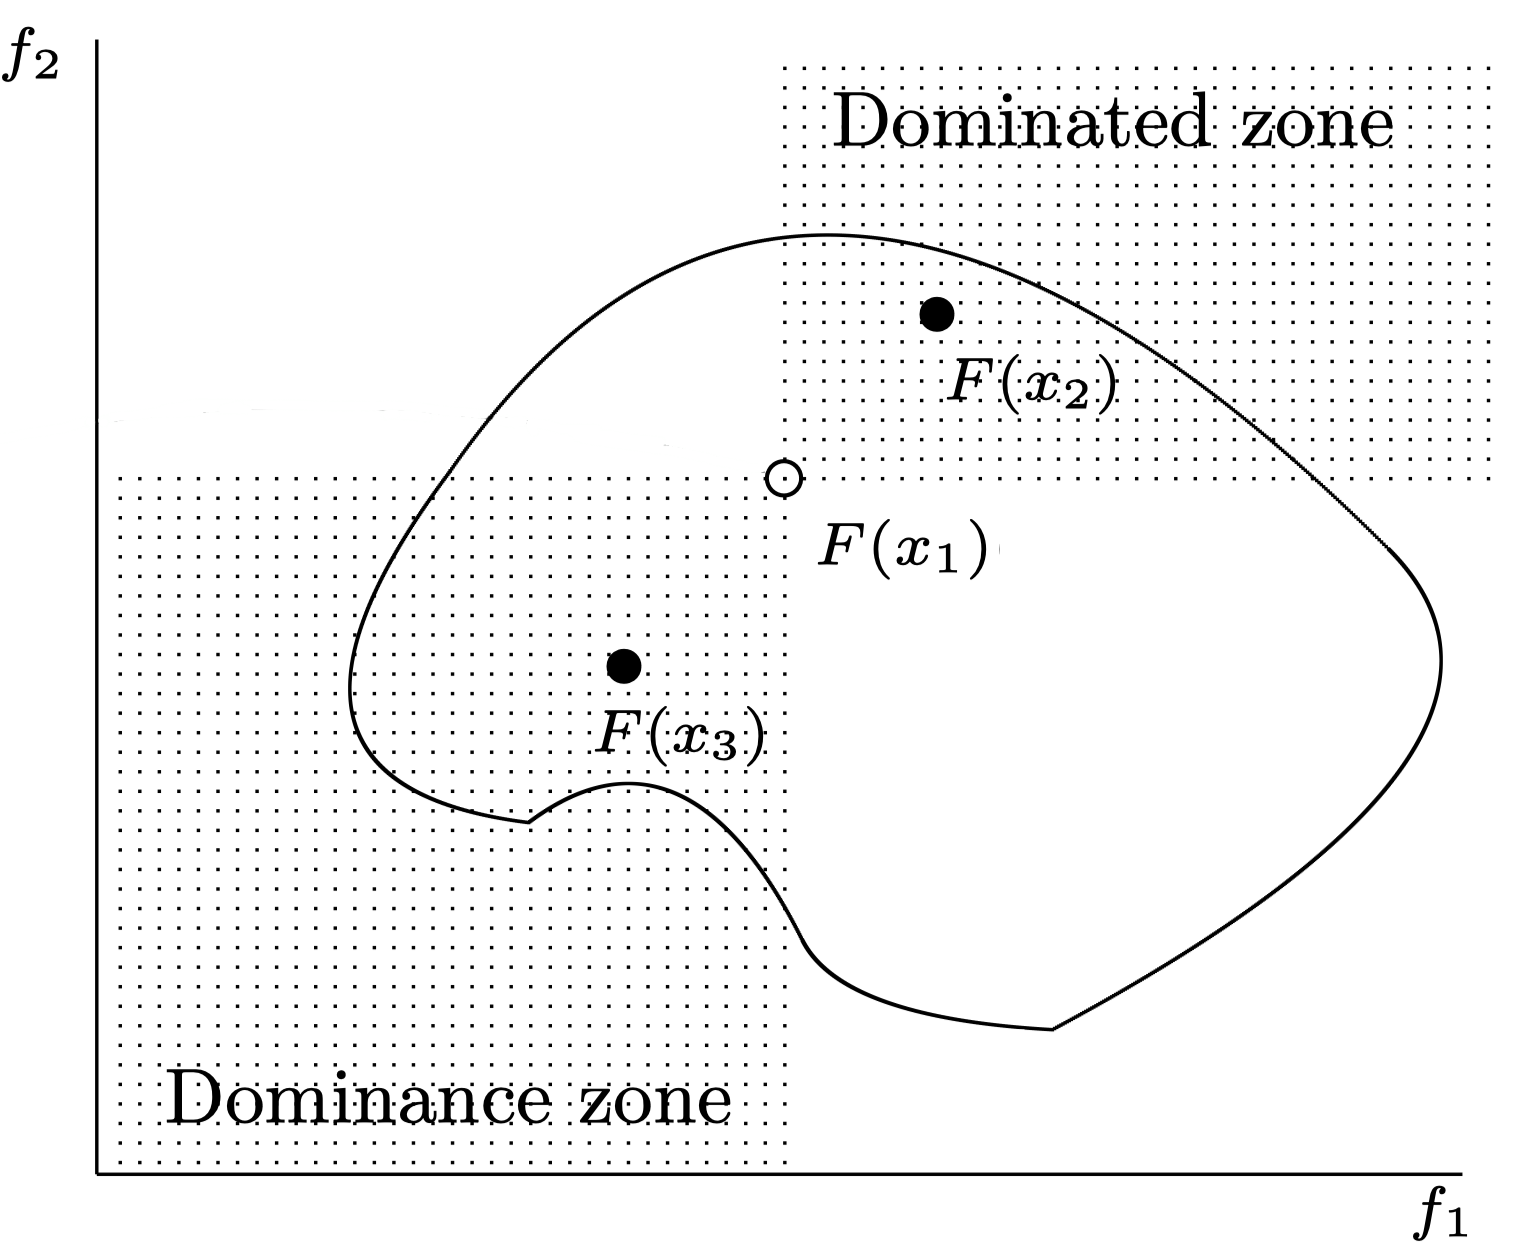
\includegraphics[width=7cm,height=5.5cm]{fig/bimadsmap.png}}
          \hspace{0.3cm} 
      \subfigure[Pareto Set]{ \label{fig:pareto_exp} 
        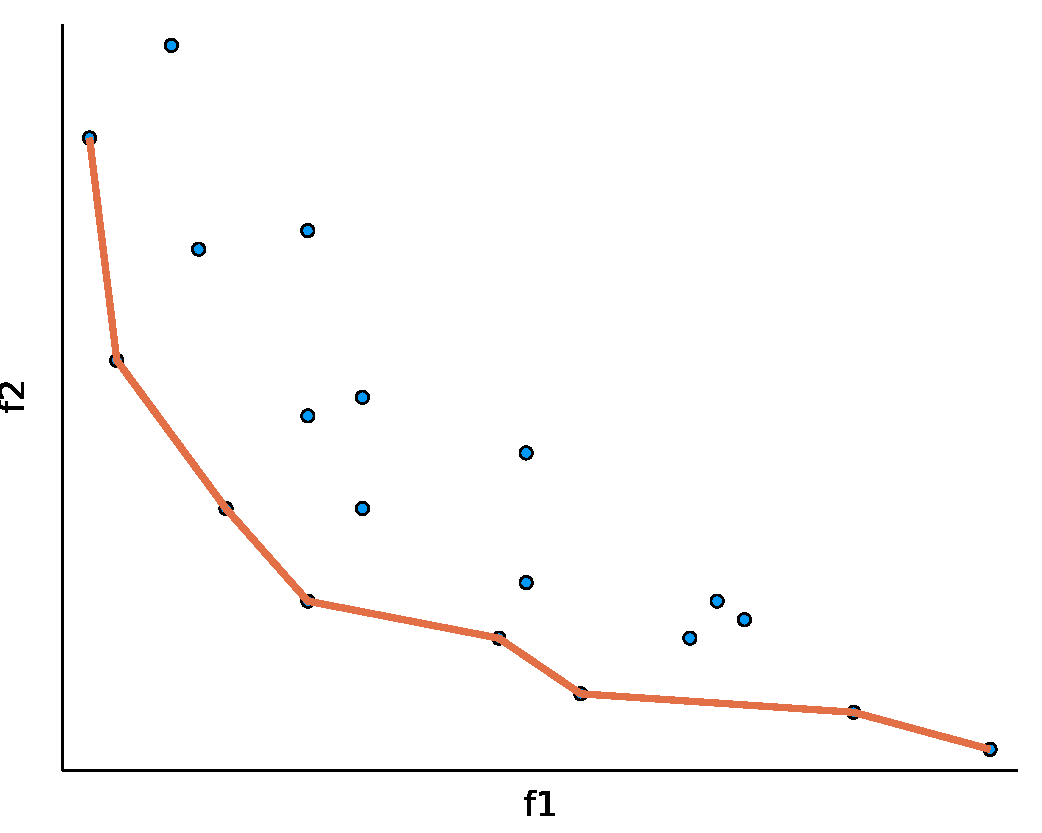
\includegraphics[width=7cm,height=5.5cm]{fig/pareto_example.pdf}}
          \caption{Illustration for Pareto dominance and set in the objective space} 
            \label{fig:pare_ill}
    \end{figure}

     Figure~\ref{fig:pare_ill} illustrates these notions with three points. In Figure~\ref{fig:domin}, $x_1$ dominates all the feasible points in the dominated zone (i.e., $x_1\prec x_2$), while it is dominated by all the points in the dominance zone (i.e., $x_3\prec x_1$). By this definition, the Pareto set can be obtained as shown in Figure~\ref{fig:pareto_exp} on the orange line.


  \subsection{Derivative-free Optimization}
    BiMADS is a derivative-free optimization algorithm that approximates the Pareto set of a bi-objective problem. It first formulates the problem into a series of single-objective problems and then solves a series of bound-constrained single-objective problems using MADS with increasingly stringent stopping criteria.

    \subsubsection*{Mesh Adaptive Direct Search (MADS)}\label{sec:MADS}
    MADS is originally proposed in~\cite{audet2006mesh}, which is a direct search method used for minimizing a non-smooth function $f: \mathbb{R}^{m} \rightarrow \mathbb{R} \cup\{+\infty\}$ within the constraint set $\Omega \subseteq \mathbb{R}^{m}$. The MADS algorithm generally has three phases for iteration $k$:
    \begin{itemize}
    \item Search Phase: Generating a set of search points using a specified search algorithm, which aims to search around the entire objective space to find the best point currently (incumbent point). 
    \item Poll Phase: Searching along with all possible directions for the given initial point or the incumbent point, to find a new dominating point for the next iteration.
    \item Update Phase: Updating the parameters such as Mesh/Frame size to enlarge or refine the search space.
    \end{itemize}

    The concepts of Mesh and Frame are essential to MADS, where the mesh size vector $\Delta^{m}_{k} \in \mathbb{R}^n$ determine the set of points that may be evaluated as trial points. The frame size vector $\Delta^{p}_{k} \in \mathbb{R}^n$ defines the search space from where the new incumbent point can be selected. Figure~\ref{fig:mesh} illustrates the mesh size, frame size and the MADS will evaluate the trail points (i.e., $p^{1,2,3}$) around the current incumbent point $x_k$ to find the new dominating point.

    \begin{figure}[H]
    \centering
    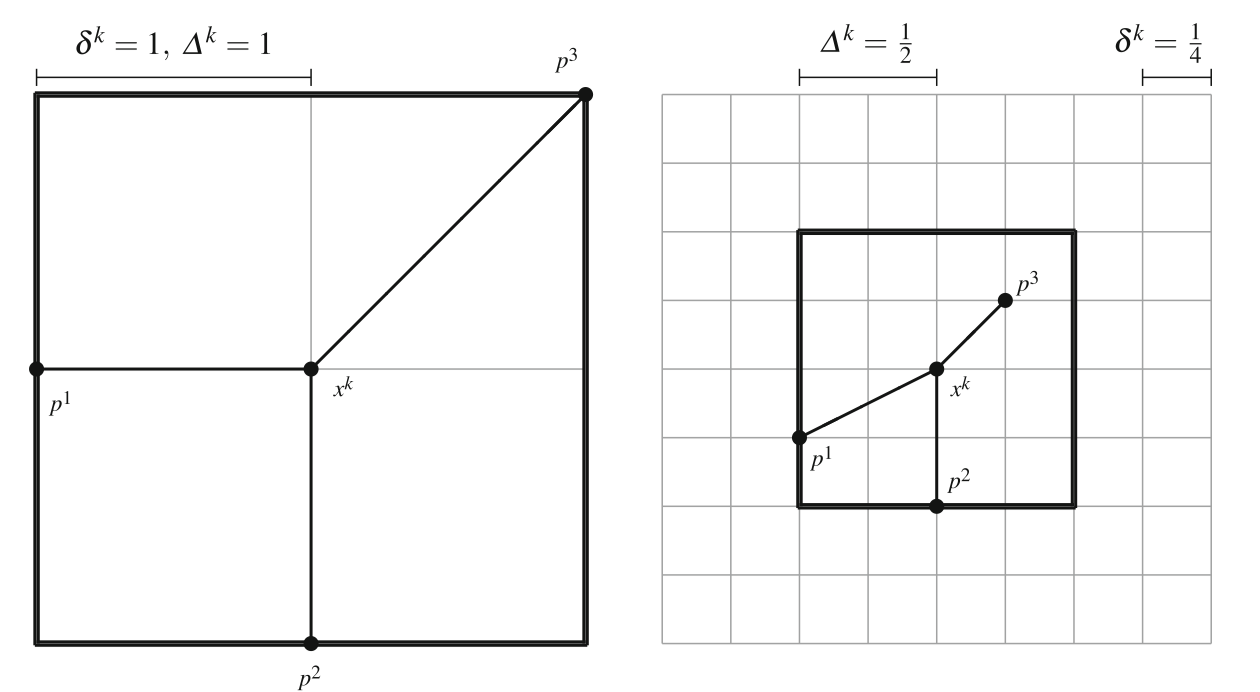
\includegraphics[width=9cm]{fig/mesh-frame.jpg}
    \caption{Examples of meshes and frames in $\mathbb{R}^{2}$ for different $\Delta^{m}_{k}$ and $\Delta^{p}_{k}$~\cite{audet2006mesh}}
    \label{fig:mesh}
    \end{figure}
     In addition, the MADS implemented in \verb|DirectSearch.jl| has been improved according to \cite{abramson2009orthomads} and \cite{audet2019mesh}, where the first one introduces the \verb|OrthoMADS| to minimize the size of the cones of unexplored directions. The latter one introduces Granular variables to solve the problems with constraints on the granularity of variables.

  \subsection{Bi-objective mesh adaptive direct search (BiMADS)}
    The original BiMADS algorithm is shown in Algorithm 1~\cite{audet2008multiobjective} and the detailed explanation for each part is also shown in this section.
    \subsubsection{Initialization}
    The BiMADS first runs the Initialization stage with a given point $x_0$. This stage minimizes two single-objective problem
    \begin{equation}
    \min _{x \in \Omega} f_{1}(x) \quad \text { and } \quad \min _{x \in \Omega} f_{2}(x)
    \end{equation}
    using MADS individually. During the optimization, all the dominating points in Search or Poll phase have to be stored and evaluated by Pareto dominance criterion to obtain the very first Pareto set $X_\mathcal{L}$ with cardinality $J$. Also, the weight for each points $w(x)$ and the weighted distance $\delta\in \mathbb{R}^J$ need to be set as above to determine the reference point.

    \subsubsection{Main Iterations}
    After obtaining the first Pareto set, the main part of the BiMADS will be run iteratively until hitting the stopping condition. The updated Pareto set will gradually approach the Pareto front and attempt a uniform coverage of the Pareto front.

    \begin{algorithm}[H]
      \caption{BiMADS Algorithm~\cite{audet2008multiobjective}}
      \begin{algorithmic}
      \State \textsc{Initialization}:
          \begin{itemize}
          \item Apply MADS from initial point $x_0$ to solve $\min _{x \in X} f_{1}(x)$ and $\min _{x \in X} f_{2}(x)$, where $X\in \mathbb{R}^n$ is the feasible set.
          \item Let $X_{\mathcal{L}}=\left\{x^{1}, x^{2}, \ldots, x^{J}\right\}$ be an ordered list of pairwise non-dominated points such that $\qquad f_{1}\left(x^{1}\right)<f_{1}\left(x^{2}\right)<\cdots<f_{1}\left(x^{J}\right)$ and $f_{2}\left(x^{1}\right)>f_{2}\left(x^{2}\right)>\cdots>f_{2}\left(x^{J}\right)$
          \item Initialize the weight $w(x)=0$ for all $x \in X$ and let $\delta>0$
      \end{itemize}
      \State \textsc{Main iteration}: Repeat
          \begin{itemize}
            \item \textsc{Reference point determination}:
              \begin{enumerate}[-]
                \item If $J>2$, let $\hat{\jmath} \in \operatorname{argmax}_{j=2, \ldots, J-1} \delta^{j}=\frac{\left\|F\left(x^{j}\right)-F\left(x^{j-1}\right)\right\|^{2}+\left\|F\left(x^{j}\right)-F\left(x^{j+1}\right)\right\|^{2}}{w\left(x^{j}\right)+1}$ and determine the reference point $r=\left(f_{1}\left(x^{\hat{\jmath}+1}\right), f_{2}\left(x^{\hat{\jmath}-1}\right)\right)$.
                \item If $J=2$, let $x^{\hat{\jmath}}=x^{2}$, determine the reference point $r=\left(f_{1}\left(x^{2}\right), f_{2}\left(x^{1}\right)\right)$ and set $\delta^{\hat{\jmath}}=\frac{\left\|F\left(x^{2}\right)-F\left(x^{1}\right)\right\|^{2}}{w\left(x^{2}\right)+1}$.
                \item If $J=1$, let $x^{\hat{\jmath}}=x^{1}, \delta^{\hat{\jmath}}=\frac{\delta}{w\left(x^{\hat{\jmath}}\right)+1}$ and apply the MADS algorithm from $x^{\hat{\jmath}}$ to solve $\min _{x \in X} f_{1}(x)$ and $\min _{x \in X} f_{2}(x)$. Terminate MADS using the same condition as in \textsc{Initialization} and continue to the step \textsc{Update} $X_{\mathcal{L}}$.
              \end{enumerate}          
            \item \textsc{Single-objective formulation minimization:}\label{sec:phi}
              \begin{enumerate}[]
                  \item Solve a single-objective formulation $\phi_r$ by MADS from the starting point $x^{\hat{\jmath}}$. Terminate MADS when the mesh size parameter $\Delta^m$ drops below $\Delta\left(\delta^{\hat{\jmath}}\right)=O\left(\delta^{\hat{\jmath}}\right)$ or if a maximal number of objective evaluations is attained.
              \end{enumerate} 
            \item \textsc{Update} $X_{\mathcal{L}}$
              \begin{enumerate}[]
                  \item Add all non-dominated points found in the current iteration to $X_{\mathcal{L}}$, remove dominated points from $X_{\mathcal{L}}$ and order the resulting list of points.
                  \item Increase weights: $w\left(x^{\hat{\jmath}}\right) \leftarrow w\left(x^{\hat{\jmath}}\right)+1$ for each $x \in X_{\mathcal{L}}$.
              \end{enumerate} 
          \end{itemize}
      \end{algorithmic} 
    \end{algorithm} 
    \subsubsection*{Reference Point Determination}\label{sec:weight}
    Firstly, the reference point $r\in \mathbb{R}^2$ should be found for the single-objective reformulation and optimization. If $J>2$, the euclidean distance between 3 successive points in the Pareto set are calculated as shown in Figure~\ref{fig:ref_det}. The points with the largest distance will be potentially selected as the reference point. The BiMADS algorithm will search around the reference point and try to fill the gap with other Pareto solutions to approach the actual Pareto front. Figure~\ref{fig:fillgap} shows the progress for each iteration. However, some bi-objective problems have discontinuous Pareto fronts naturally as shown in Figure~\ref{fig:dt2}. Hence the BiMADS will stall near these break-points and waste time on searching for nothing. Therefore, a weight should be associated with each point to count the number of being the reference point and the point $j$ with the largest weighted distance $\delta^j$ will be selected to generate the reference point. If $J=2$, then the second point is selected. If $J=1$, then we repeat the Initialization with the new initial point $x^1$.

    \begin{figure}[H] 
    \centering 
      \subfigure[Construction of Reference point~\cite{audet2008multiobjective}]{\label{fig:ref_det}
        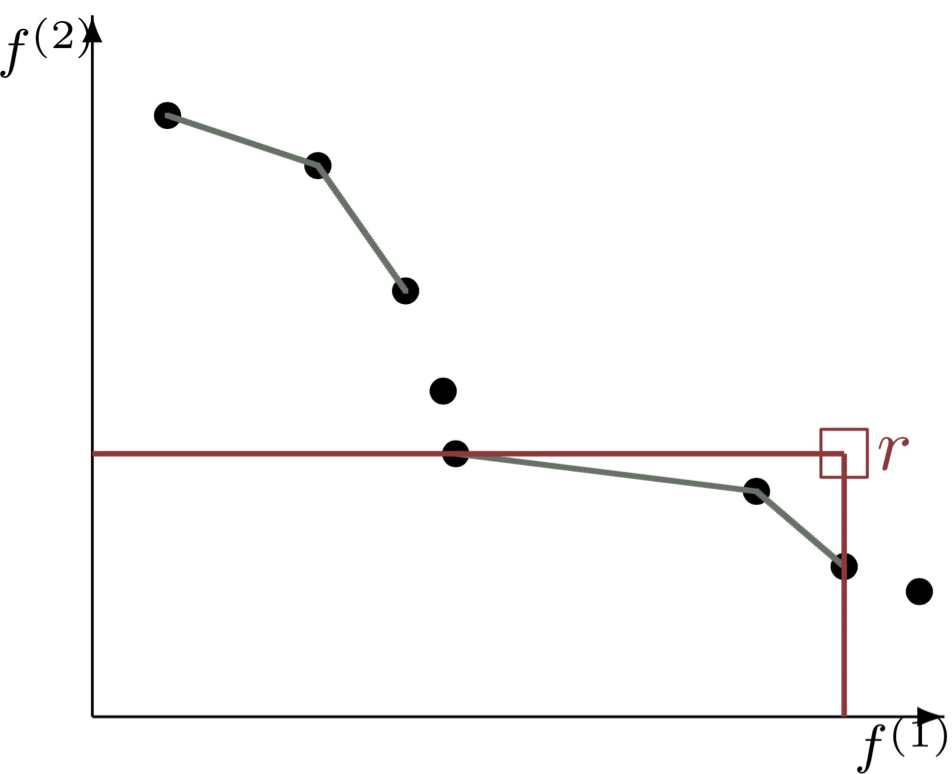
\includegraphics[width=7.5cm,height=6cm]{fig/ref.jpg}}
          \hspace{0.3cm} 
      \subfigure[Discontinuous Pareto front]{ \label{fig:dt2} 
        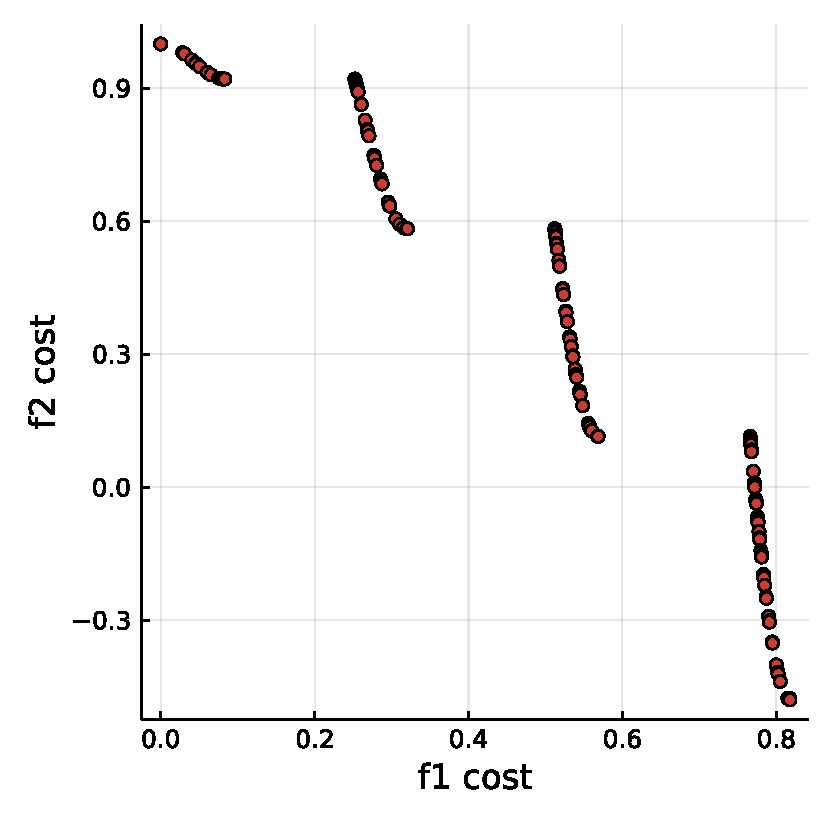
\includegraphics[width=7.5cm,height=6cm]{fig/dt2.pdf}}
          \caption{Illustration for reference point determination and natural gaps in Pareto front} 
            \label{fig:refall}
    \end{figure}

    \subsubsection*{Single-objective formulation minimization}
    After obtaining the reference point $r\in \mathbb{R}^2$ associated with Pareto solution $x^j$, the then bi-objective problem could be reformulated as single-objective problem 
    \begin{equation}\label{equ:reform}
    \min _{x \in \Omega} \phi_{r}(F(x)),
    \end{equation}
    where $\phi_{r}:\{\mathbb{R} \cup\{+\infty\}\}^{2} \rightarrow \{\mathbb{R} \cup\{+\infty\}\}$ is
    \begin{equation}
    \phi_{r}(s):= \begin{cases}-\left(r_{1}-f_{1}(x)\right)^{2}\left(r_{2}-f_{2}(x)\right)^{2} & \text { if } f_{1}(x) \leq r_1\ \text{and}\ f_{2}(x) \leq r_2 \\ \left(\max \left\{f_{1}(x)-r_{1}, 0\right\}\right)^{2}+\left(\max \left\{f_{2}(x)-r_{2}, 0\right\}\right)^{2} & \text { otherwise. }\end{cases}
    \end{equation}

    \noindent Under this reformulation, the level set of $\phi_{r}$ is shown in Figure~\ref{fig:level}. The values of $\phi_{r}$ are negative if and only if the trial points are in the dominance zone of $r$. Otherwise, $\phi_{r}\geq0$. Then in each iteration, the MADS will be applied to the problem in Equation~\eqref{equ:reform}, which will try to evaluate trial points lying in the dominance zone of $x^j$ and attempt to fill the gap as shown in Figure~\ref{fig:bimads1}. Similarly, all the dominating points for this MADS optimization should be added to $X_\mathcal{L}$. The convergence analysis is detailed in~\cite{audet2008multiobjective}.
    \begin{figure}[h] 
    \centering 
      \subfigure[Level set of $\phi_{r}$]{\label{fig:level}
        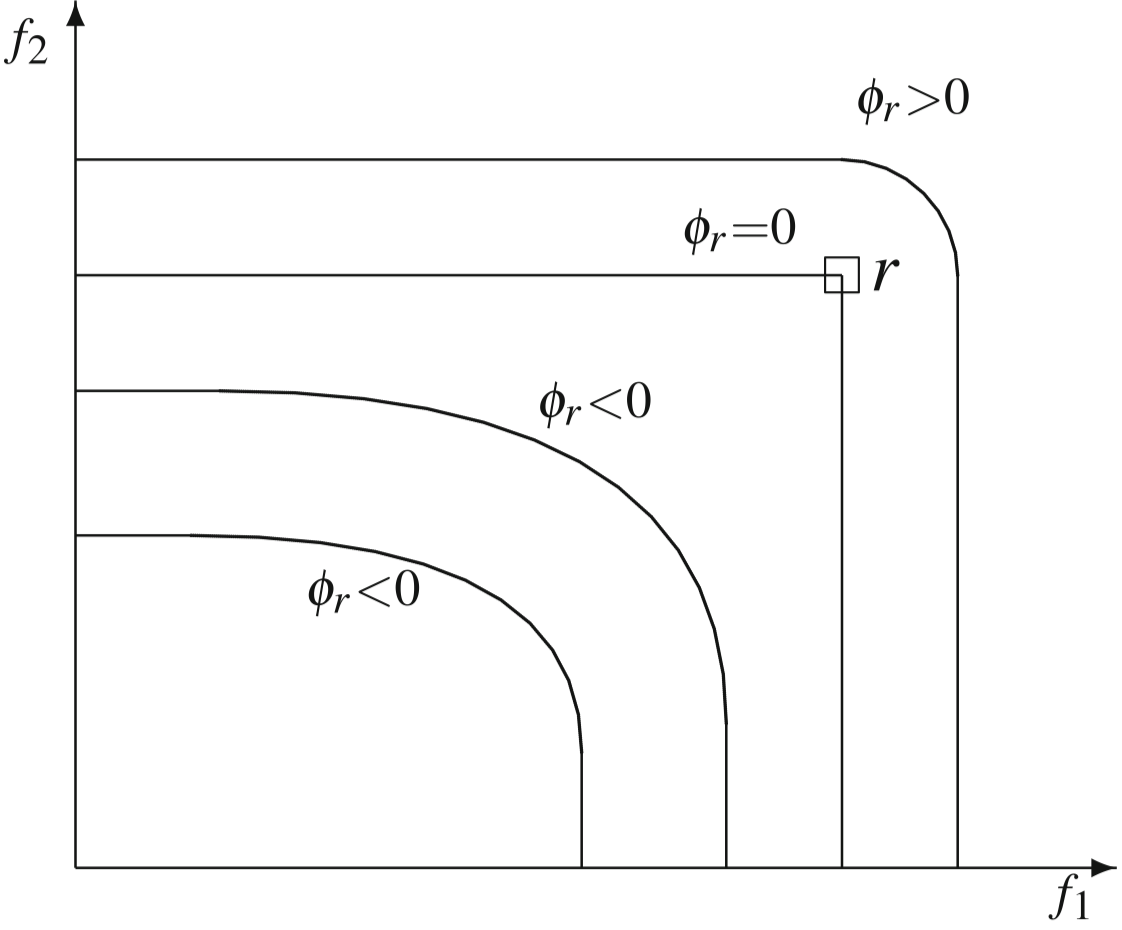
\includegraphics[width=7.5cm,height=6cm]{fig/level.jpg}}
          \hspace{0.3cm} 
      \subfigure[Trail points in dominance zone]{ \label{fig:bimads1} 
        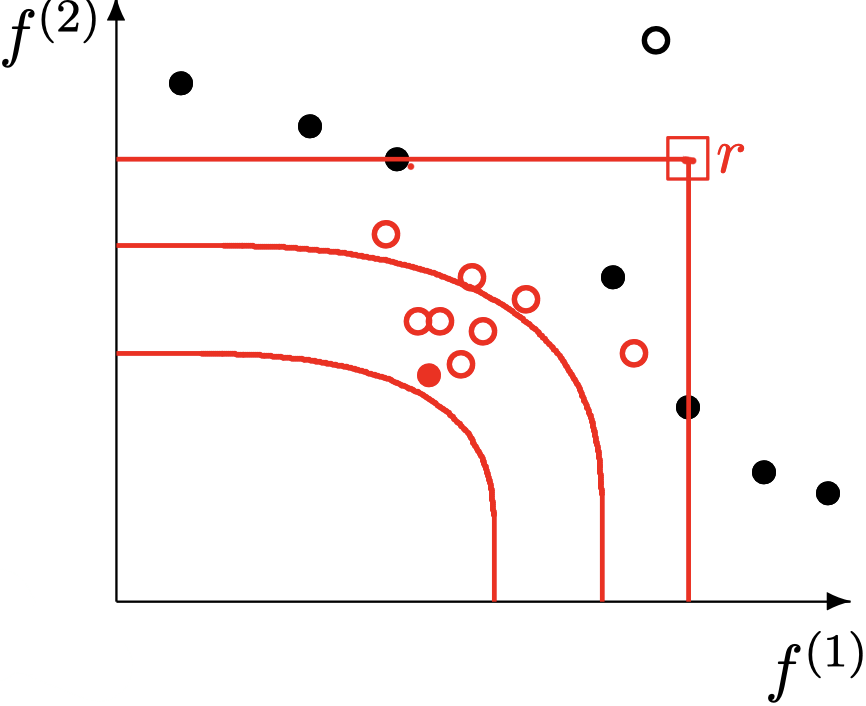
\includegraphics[width=7.5cm,height=6cm]{fig/bimads1.jpg}}
          \caption{Illustration for problem reformulation~\cite{audet2017derivative}} 
            \label{fig:reform}
    \end{figure}
    \subsubsection*{Update $X_\mathcal{L}$}
    At the end of each iteration, the BiMADS will remove all the dominated points in $X_\mathcal{L}$ with only Pareto solutions left. The weight associated with the current selected point $x^j$ should also be increased by 1 to presenting stalling for some problems with discontinuous Pareto fronts.

    The original BiMADS algorithm only supports two stopping conditions. The optimization will be terminated either after a fixed number of BiMADS iterations or when the $\delta^{\hat{\jmath}}$ is lower than a pre-set threshold. However, more stopping conditions is required to gain more flexibility for solving some complex problems, which will be explained in Section~\ref{sec:stop}.

  \subsection{Software Packages for BiMADS}
    \subsubsection*{NOMAD in C++}
    The original BiMADS algorithm and some improvements~\cite{audet2019mesh,abramson2009orthomads} have been implemented in \verb|NOMAD-3.9| in C++~\cite{le2011algorithm}. This package is developed by the group who proposed MADS/BiMADS but it does not provide enough flexibility on modifying the parameters to adapt to different problems. In this project, \verb|NOMAD-3.9 C++| will be used as a benchmark to evaluate the performance of BiMADS in \verb|DirectSearc-| \verb|h.jl|. The aim is to achieve a similar or better performance while providing more flexibility on customizing the optimizations.

    \subsubsection*{DirectSearch.jl}
    The current version of \verb|DirectSearch.jl| was developed by Edward Stables~\cite{originalMADS} and Lukas Baliunas~\cite{originalMADS2}, and only support single-objective optimization using MADS. This package leverages Julia's features such as multiple dispatch and abstract type to speed the optimization and simplify the code structure. Here are some important types with their hierarchy relations and functionalities.
    \begin{itemize}
    \item \verb|DSProblem| inherit from \verb|AbstractProblem|, which is used to define the problems to be optimized. The members of this type includes objective functions, constraint functions, initial points, stopping conditions, iteration/evaluation limitations, current feasible solution and cost.
    \item \verb|Status|, \verb|Config| are two concrete types and instantiated in \verb|DSProblem|. They store the configuration options and status information for the solver, such as current mesh/poll size, direction, iteration number.
    \item \verb|AbstractStoppingCondition| is an abstract type and cannot be instantiated. It contains all the concrete types for stopping condition such as \verb|IterationStoppingCondition|, \\\verb|MeshPrecisionStoppingCondition| etc. These different concrete types make it possible to dispatch the same function for evaluating different stopping conditions.
    \end{itemize}

   In this project, BiMADS will be added into \verb|DirectSearch.jl| as an extension. All the types mentioned above will be used for the same purpose as in MADS. Several new types will also be introduced in Section~\ref{sec:stop}.

  \subsection{Evaluation Method}
  \subsubsection*{Hypervolume Indicator}
  Hypervolume indicator~\cite{zitzler1998multiobjective} is a common way to assess the quality of Pareto sets obtained from multi-objective optimizations. It calculates the volume of the objective space dominated by a Pareto set and delimited above by a reference point $r\in \mathbb{R}^p$, where $p$ is the number of the objective functions. Figure~\ref{fig:hv} illustrates the hypervolume for bi-objective space, which is the area enclosed by all the Pareto solutions and the reference point. Furthermore, to normalize the numerical value of hypervolume, the actual area is divided by the triangle area enclosed by the ideal point and two endpoints as shown in Figure~\ref{fig:hv}.
  \begin{figure}[t]
  \centering
  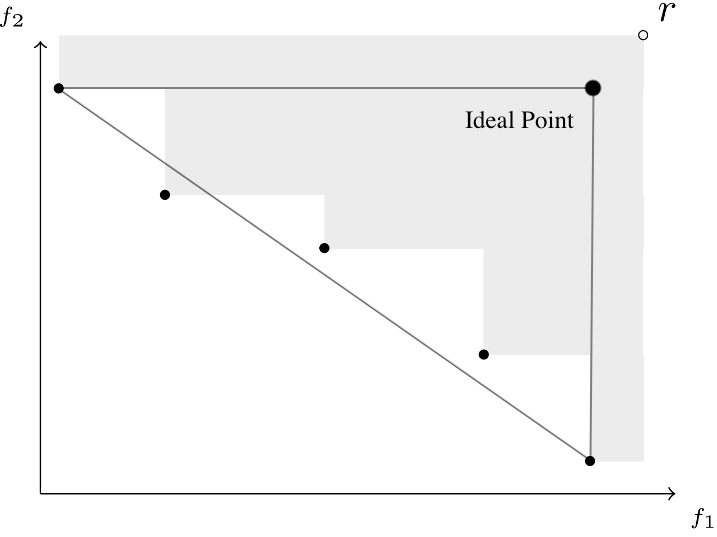
\includegraphics[width=8cm]{fig/hv_eg.png}
  \caption{Hypervolume Indicator for bi-objective problems~\cite{bigeon2021dmulti}}
  \label{fig:hv}
  \end{figure}
  According to \cite{ishibuchi2018specify}, the selection of the reference point affects the performance of the indicator, hence the performance of the optimization algorithms. Some of the points may have low hypervolume contributions, which means the hypervolume will not be decreased much without them. These points might be neglected, hence the Pareto set will be non-uniformly distributed. \cite{ishibuchi2018specify} suggest selecting the reference point $k$ times away from the ideal point (in terms of each dimension) to ensure each Pareto solution has the same hypervolume contributions. Here, $k=1+1/\mu$, where $\mu$ is the number of the points in the Pareto set.

  \subsubsection*{Performance Profile}
  To compare the performance between \verb|NOMAD| and \verb|DirectSearch.jl|, the Julia package \verb|BenchmarkPr-| \verb|ofiles.jl| will be used~\cite{dolan2002benchmarking}. It is based on the performance profile, which describes the (cumulative) distribution function for a performance metric. The package will take the cost (i.e., run time, iteration number) of all the solvers for different optimization problems. Then, for each problem, the best cost will be selected as the baseline to carry out the comparison. Finally, the package will output a figure which describes the proportion of the problems that can be solved by the solver within a factor $\tau$ of the best solver.
  \subsubsection*{Unit Test}
  Unit test is necessary for any software development. It aims to ensure that each unit in the software could provide the proper result as expected. Each unit test function will test a small unit (i.e., functions, objects) that can be logically isolated in a package or system and verify its correctness~\cite{zhu1997software}. The main advantages of implementing the unit test can be concluded as
  \begin{enumerate}
  % \item Even a small change may crush the whole system. Thus, the unit test could validate all the functions right after making changes. In other words, i
  \item Unit test helps the developers to refactor codes or work on some unfamiliar codes because they can identify the bugs easily and quicker.
  \item Unit test could serve as documentation. It helps new developers to learn the functionality provided by each unit. Also, it provides an appropriate or inappropriate usage of a function or module.
  % \item Unit test helps the developers to design each unit in a clever way because they need to think through the design and specify the functionality for each unit. Besides, if the unit test is designed in a cumbersome manner (i.e., too many if-else), the developers may need to simplify the code for better performance.
  \end{enumerate}

  Julia provides a package called \verb|Test.jl| to implement basic unit test using the following macros:
  \begin{itemize}
  \item \verb|@testset| groups tests into a set.
  \item \verb|@test| tests that if the expression evaluates to \verb|true|.
  \item \verb|@test_throw| tests that if the expression throws an exception/error.
  \end{itemize}

  Figure~\ref{fig:test_fail} shows an example of a failed unit test, where two failures occur in the test set named \verb|Optimization for p1 and p2|. Thus, the users can quickly locate the bugs. As for this project, a test file will be design to test all the new implementations and all the tests should be passed in the final deliverable package.
    \begin{figure}[htp]
  \centering
  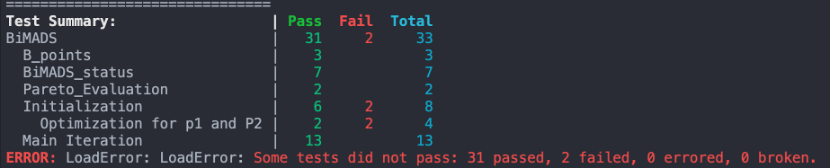
\includegraphics[width=14cm]{fig/test_fail.png}
  \caption{Result of a failed unit test}
  \label{fig:test_fail}
  \end{figure}

\section{Design and Implementation}\label{sec:ana}
  This section provides the short requirements analysis, code structure design and code implementation for extending \verb|DirectSearch.jl| with BiMADS algorithm, which is also the most important requirement of this project. The design will be explained in three parts: problem formulation, initialization and main BiMADS iteration. In addition, the explanations for different stopping conditions and unit test will also be detailed. All the new implementations can be found on \href{https://github.com/amazing0844/DirectSearch.jl}{\textcolor{blue}{GitHub}}.
  \subsection{BiMADS}
  \subsubsection{Problem Formulation}
  In \verb|DirectSearch.jl|, an optimization problem is defined by an instance of \verb|DSProblem|, where users could set the parameters such as numbers of variables, iteration limits, initial points, granularity, and most importantly the objective function(s). As for the original code, the expression for the function is written in a \verb|function| with \verb|Float64| as the return value.

  However, BiMADS problems will have two objective functions. Meanwhile, the mathematical expressions are required for both functions instead of two \verb|Float64| numbers because these functions will be optimized by MADS separately in the initialization stage. Therefore, a new formulation structure is used for BiMADS as
  \begin{minted}[breaklines,escapeinside=||,mathescape=true, linenos, numbersep=3pt, gobble=2, frame=lines, fontsize=\small, framesep=2mm]{julia}
  function obj(x)
      f1(x) = ...
      f2(x) = ...
      return [f1,f2]
  end
  \end{minted}
  The users need to define a \verb|function obj(x)| which contains two functions with \verb|Float64| returned. The \verb|obj(x)| returns a \verb|Vector{function}| and will be passed to the instance of \verb|DSProblem|. Then, this instance will be passed to \verb|Optimize!|, which is the only public API for the optimization. To distinguish between single and bi-objective problems, the dimension of \verb|obj(x)| needs to be assessed by the function \verb|p_dim|. Finally, the bi-objective problems will be solved by \verb|Optimize_Bi!|, where the actual BiMADS algorithm implements.

  \subsubsection{Initialization}
  The flow chart for initialization stage is shown in Figure~\ref{fig:flow_init} which follows the \textsc{Initialization} part in  Algorithm 1.
  \begin{figure}[t] 
  \centering 
      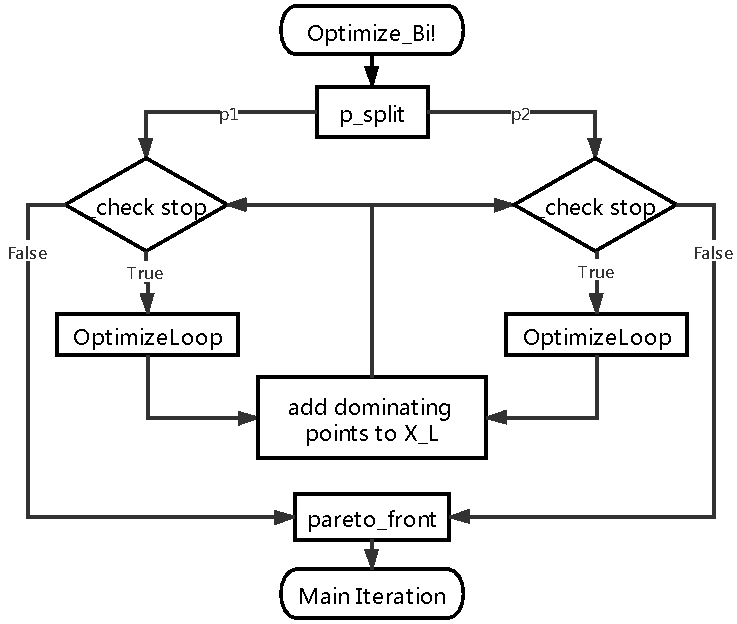
\includegraphics[width=14cm]{fig/initialization.pdf}
        \caption{Flow chart for Initialization} 
    \label{fig:flow_init} 
  \end{figure}
  To explain:
  \begin{enumerate}
    \item The bi-objective \verb|DSProblem| instance \verb|p| is firstly split into \verb|p1| and \verb|p2| by function \verb|p_split|, where both \verb|p1|, \verb|p2| are instances with single-objective function \verb|f1| and \verb|f2|.
    \item \verb|p1| and \verb|p2| will be optimized using MADS algorithm individually to find their optimum solutions. During the optimizations, if the current MADS iteration is labeled as \verb|dominating iteration|, which means a new better point with smaller cost is found as the new incumbent point. 
    \item A new type named \verb|B_points| was designed as shown in List~\ref{lis:bpoints} to store the following information. Firstly, the current solution $x$ should be stored along with its costs in terms of \verb|f1| and \verb|f2| in line 1 and 2. These two costs will be used as a coordinate to identify a point in 2D objective space. In addition, as mentioned in Section~\ref{sec:weight}, all the points should be associated with a weight for the reference point determination stage as in line 3. Also, the new type contains a inner constructor to create an instance for this type.

    \begin{listing}[ht]
      \begin{minted}[breaklines,escapeinside=||,mathescape=true, linenos, numbersep=3pt, gobble=2, fontsize=\small, framesep=2mm]{julia}
    """
    points for BiMADS Algo in objective space
    """
    mutable struct B_points
        cost::Vector{Float64} #f1 and f2 value in objective space
        x_now::Vector{Float64}# current variable
        weight::Int           #weight for each undominated point to determine $\delta$
        function B_points(cost::Vector{Float64},x::Vector{Float64}, w::Int=0) #inner constructor
            p = new()
            p.cost = cost
            p.x_now=x
            p.weight = w
            return p
        end
    end
    \end{minted}
  \cprotect\caption{A new type named \verb|B_points|}
  \label{lis:bpoints}
  \end{listing}
      Then, all the points in objective space can be stored in a \verb|Vector{B_points}| set $X_\mathcal{L}$ for later usage.
      \item The last step is to evaluate all the points using function \verb|pareto_front| to find the Pareto set. The general design for this function is to filter out all the dominated points and sort the rest of them for the reference point determination.
  \end{enumerate}

  In addition, if the iteration or function evaluation limit have already been run out in the initialization stage, an error will be thrown out to warn the users to provide more budgets for iteration or function evaluation limits so that the initialization stage could be finished.

  \subsubsection{Main Iteration}
  The flow chart for main iteration stage is shown in Figure~\ref{fig:flow_main} which follows the \textsc{Main iteration} part in Algorithm 1.
  \begin{figure}[t] 
  \centering 
      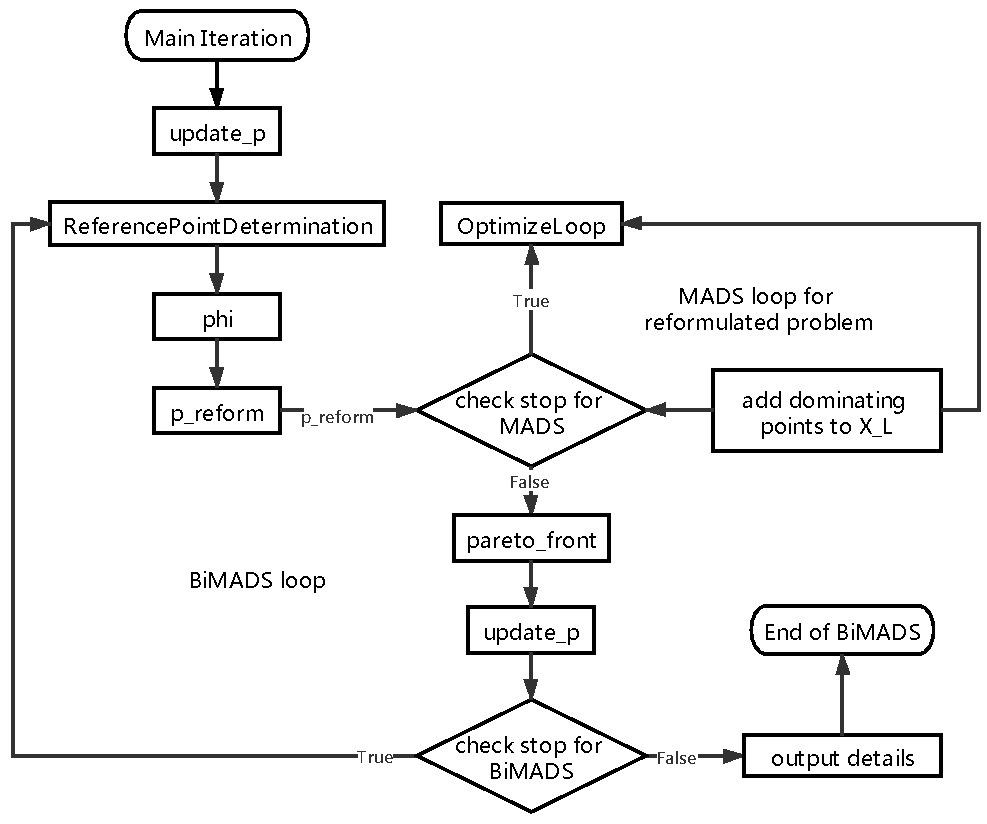
\includegraphics[width=16cm]{fig/main_iter.pdf}
        \caption{Flow chart for Main Iteration} 
    \label{fig:flow_main} 
  \end{figure}

  To explain, before entering the BiMADS loop, a new instance of \verb|DSProblem| called \verb|p_reform| should be initialized for the reformulated single-objective problem for $\phi_r$. \verb|p_reform| is a copy of the very first bi-objective problem instance \verb|p| because most of their parameters are the same, such as stopping conditions. The only differences are the objective function and initial point which will be set later. The initialization stage also has already spent some iteration and function evaluation budgets. Therefore, the value of these two parameters should be subtracted from the total budgets in \verb|p_reform| by function \verb|update_p|.

    In addition, the MADS for \verb|p_reform| are nested in the BiMADS loop. However, their stopping conditions are almost the same. For instance, both of these algorithms will be terminated once reaching the iteration limit. Therefore, a new type is designed and implemented to store the BiMADS optimization status as shown in List~\ref{lis:status}, with comments for each member in the type. The status for MADS optimization will still be stored in the \verb|p.status|, which is a member with type \verb|status| in \verb|DSProblem|.
        \begin{listing}[ht]
      \begin{minted}[breaklines,escapeinside=||,mathescape=true, linenos, numbersep=3pt, gobble=2, fontsize=\small, framesep=2mm]{julia}
  """
  Status for BiMADS main iteration, also contain stopping conditions

  """
  mutable struct BiMADS_status
    iteration::Int64                #Total iteration spent
    func_evaluation::Int64          #Total function evaluation spent
    total_time::Float64             #Total running time
    hypervolume::Float64            #Hypervolume for current Pareto set
    opt_status::OptimizationStatus  #one of the stopping condition
    opt_string::String              #string for the condition above
    start_time::Float64             #start time for the optimization
    function BiMADS_status()        #inner constructor
        s=new()
        s.iteration=0
        s.func_evaluation=0
        s.total_time=0.0
        s.hypervolume=0.0
        s.opt_status=Unoptimized
        s.opt_string="Unoptimized"
        s.start_time=time()
        return s
    end
  end
    \end{minted}
  \cprotect\caption{A new type named \verb|BiMADS_status|}
  \label{lis:status}
  \end{listing}

  Then, the following steps all need to be run repeatedly.
  \begin{enumerate}
    \item The function \verb|ReferencePointDetermination| will be called to determine the reference point for the current iteration. If the cardinality of $X_\mathcal{L}$ is larger than 2, the function calculates the weighted euclidean distance between three successive points and selects the group with the largest value to determine the reference point. Otherwise, the first point is selected. Also, the initial point for the reformulated problem can be obtained as the middle point ($x^j$) from the selected group.
    \item The next step is to construct the $\phi_r$ by the function \verb|phi|. The cost for each function should be calculated and stored in advance because the calculations for some objective functions might be extremely time-consuming. Then, the $\phi_r$ and $x^j$ can be set as the objective function and initial point for the pre-constructed instance \verb|p_reform|, using the provided API \verb|SetObjective| and \verb|SetInitialPoint|.
    \item Afterwards, the \verb|p_reform| is optimized by MADS with the normal search/poll step and stopping conditions. Similarly, the \verb|x| value of all the \verb|dominating iteration| should be stored along with their \verb|f1|, \verb|f2| cost in the set $X_\mathcal{L}$. This set needs to be evaluated by the function \verb|pareto_front| to obtain the Pareto set.
    \item After finishing the MADS for $\phi_r$, the function \verb|update_p| should be called again to update iteration and function evaluation limits during the main iteration loop. However, different from the \verb|update_p| before the main iteration loop, the BiMADS optimization status also needs to be updated. Therefore, multiply dispatch, one of Julia's unique feature, is applied to share the same namespace for different but similar functionalities. The compiler will distinguish them in terms of different combination of arguments. For example, the first function in List~\ref{lis:dispatch} has four arguments as inputs while the second one has three. The Julia compiler will call the corresponding function in terms of different numbers or types of inputs.

        \begin{listing}[ht]
      \begin{minted}[breaklines,escapeinside=||,mathescape=true, linenos, numbersep=3pt, gobble=2, fontsize=\small, framesep=2mm]{julia}
    function update_p(p, p1::DSProblem, p2::DSProblem, status::BiMADS_status)
    #before Main Iteration Loop
    end
    function update_p(p_init::DSProblem, p_reform::DSProblem, status::BiMADS_status)
    #during Main Iteration Loop
    end
    \end{minted}
  \caption{Multiple dispatch in Julia}
  \label{lis:dispatch}
  \end{listing}
    \item The design and implementations of the stopping conditions will be detailed in Section~\ref{sec:stop}.
  \end{enumerate}

  Once terminating the BiMADS, several useful information will be presented, such as numbers of non-dominated points (Pareto solutions), total iterations and function evaluations, total running time, hypervolume of the Pareto set and the termination reason. All the points in the Pareto set along with their \verb|f1|, \verb|f2| cost can be obtained as the returned value of function \verb|Optimize!|.

  \subsection{Stopping Condition}\label{sec:stop}
  Five stopping conditions have been implemented in BiMADS in \verb|DirectSearch.jl| as: 
  \begin{itemize}
    \item Iteration limit for total MADS iteration (iterations spent for $p1$, $p2$ and $\phi_r$)
    \item Function evaluation limit for total MADS function evaluations (same as above)
    \item Running time limit
    \item Hypervolume limit
    \item Key interrupt
  \end{itemize}

  The last three conditions are unique for \verb|DirectSearch.jl| and not implemented in \verb|NOMAD|. The designs for the first four BiMADS stopping conditions follow the same structure as in old \verb|DirectSearch.jl|, where three functions are required for each stopping condition:
  \begin{enumerate}
    \item Function \verb|init_stoppingcondition| is called for the current condition to check that if the users defined limit number is legal (i.e., running time limit should be positive).
    \item Function \verb|CheckStoppingCondition| checks if the current status violates the corresponding limit.
    \item Function \verb|StoppingConditionStatus| returns a string that is the name of the current stopping condition.
  \end{enumerate}
  The multiple dispatch is used again because although these functions have the same goal, but they will have different internal structures for different conditions. Therefore, to implement multiple dispatch, a series of types are required as the concrete types of \verb|AbstractStoppingCondition|. \verb|DirectSearch.jl| already has the types for the first two conditions. Thus, the new types for BiMADS are \verb|RuntimeStopping-| \verb|Condition| and \verb|HypervolumeStoppingCondition|. 

  As for the internal design of the function \verb|CheckStoppingCondition|, the values for current running time and hypervolume are stored in the type \verb|BiMADS_status|. Hence, these functions only compare the values between current status and limits and return \verb|false| once the optimization reaches the maximum time or expected hypervolume. In addition, here are two clarifications for the hypervolume stopping condition:
  \begin{enumerate}
    \item Two criteria could be used to terminate the optimization: 1) achieve the expected hypervolume, 2) the improvement for the hypervolume is lower than a threshold in terms of one or more iterations. However, during the tests, the author found that BiMADS algorithm will naturally stall in some iterations, which is also found in~\cite{bigeon2021dmulti}. For example, in Figure~\ref{fig:fillgap}, the first two iterations do not contribute much to the hypervolume. In contrast, the iteration 3-5 generate much more points. In this case, the optimization will be terminated at some stage due to the stalling phenomenon. Therefore, in the current implementation, the first criterion is applied. However, it requires the users to have at least a rough guess about the expected hypervolume.
    \item The user-defined hypervolume limit cannot be achieved precisely with the same value. The reason is that the hypervolume gained in each iteration is out of control. Therefore, the final hypervolume that users get might be slightly larger than the pre-set value.
  \end{enumerate}

  The default stopping conditions for BiMADS are only key interrupt, iteration and function evaluation limits, while the other two should be added manually. These conditions could be added using \verb|AddStopping-| \verb|Condition|.

  The key interrupt stopping condition is necessary because for some time-consuming optimization problems, the users normally have little knowledge of the required time/limits. It is also too expensive to take several trials as experiments. Therefore, the key interrupt function provides a manner to stop the optimization whenever the users want (i.e., when the hypervolume does not change for a long time). Meanwhile, comparing to \verb|CTRL+c|, the codes after the optimization can be executed as well. This functionality is realized by monitoring the read-eval-print loop (REPL, an interactive command-line in Julia) from the beginning of the optimization. The BiMADS will check the REPL in each iteration as below and terminates the optimization after receiving the letter ``q'' as an input.

  \subsection{Unit test}
  The general structure for the unit test design is shown in Figure~\ref{fig:test_tree}. All the functions implemented for BiMADS have been considered and test directly or indirectly. The design of the test for each function is similar. The following part will describe the common ideal with three examples.

  \begin{enumerate}
  \item The function for checking iteration limit is tested directly by setting the limit to 1000 and checking if the optimization terminates after then. Meanwhile, function \verb|update_p| are tested indirectly because the test will not pass if \verb|update_p| makes a mistake.
  \item The auxiliary function $\phi_r$ and the reference point determination function are tested by a set of giving numerical values. The outputs are then compared with the correct answers calculated by hand.
  \item The error information also should be tested when something is wrong. For the initialization stage, the iteration limit is set to 10. Then, the error information is expected to be thrown to warn the users.
  \end{enumerate}
    \begin{figure}[t]
    \centering
    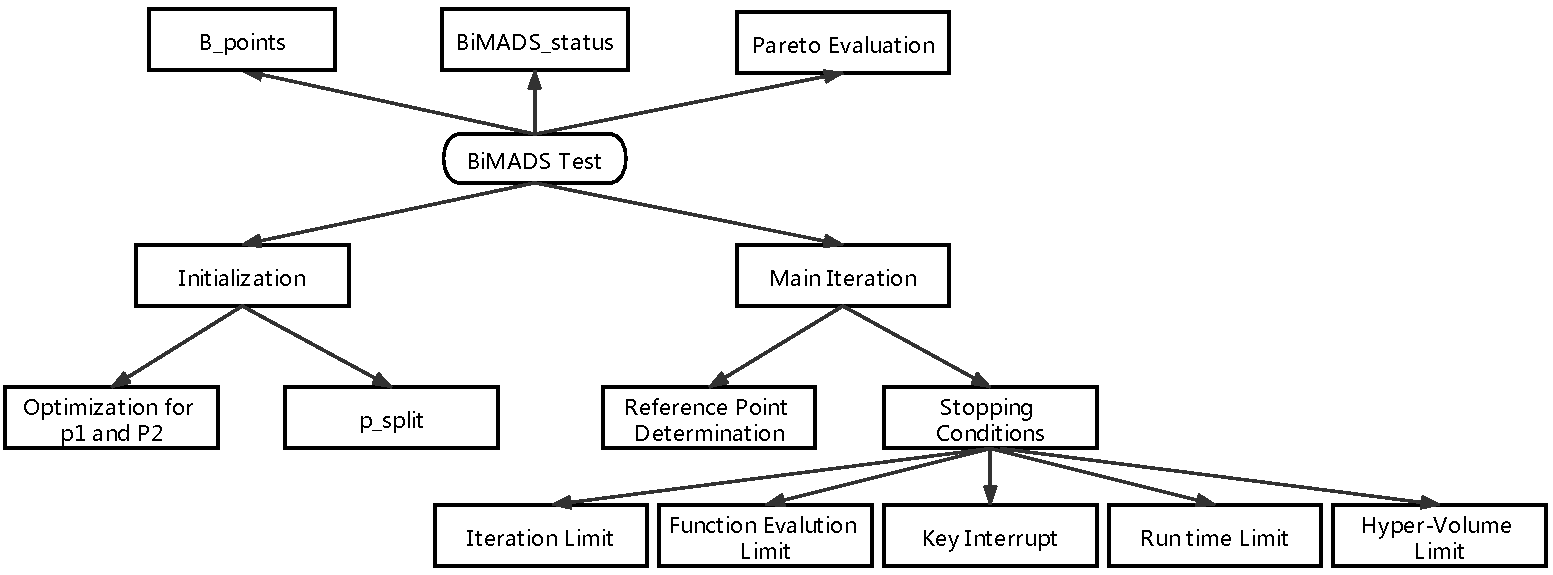
\includegraphics[width=16cm]{fig/test_tree.pdf}
    \caption{Unit test tree}
    \label{fig:test_tree}
    \end{figure}

\section{Test Problems}\label{sec:test}
  The developed package is tested on a building case study and a bi-objective problem set. This section will first introduce the modelling process for the building case. Then, the details for each optimization problem will also be provided. The codes in this section are also on \href{https://github.com/amazing0844/test_julia}{\textcolor{blue}{GitHub}}.
  \subsection{Building Case Study}\label{sec:building}
  \subsubsection{General description}
  The aim of the building case is to design a PID controller to ensure the internal building temperature follows the desired set-point and is robust to the external disturbance. The dynamic of the temperature $T(t)$ in the building is given by 
  \begin{equation}\label{equ:temp}
  \dot{T}(t)=A T(t)+c(t)+d(t),
  \end{equation}
   where:
  \begin{itemize}
    \item $A$ is a constant (see details in Appendix~\ref{sec:parameter}).
    \item $c(t)$ is the heat delivered to the flat, which is also the output of the PID controller.
    \item $d(t)=-AT_{ext}$ describes the disturbance function, where $T_{ext}$ is the external temperature variation.
  \end{itemize}
  The objectives for the case are formulated as:
  \begin{itemize}
    \item Minimize the Integrated Absolute Error (IAE) between the current building internal temperature $T(t)$ and the pre-set temperature $T_r(t)$ as 
    \begin{equation}
  \int_{0}^{T f}\left|T(t)-T_{r}(t)\right| \mathrm{d} t.
  \end{equation}\label{equ:dist}
    \item Minimize the maximum sensitivity 
      \begin{equation}
  M_{s}=\max_{\omega}|S(j \omega)|
  \end{equation}
     to external disturbance, where $S(s)=\frac{P(s)}{1+P(s) C(s)}$. $M_s$ tells the worst-case amplification of the disturbances and $P(s),\ C(s)$ are the transfer function for the system and controller respectively. The controller is designed to minimize the maximum absolute value of $S(j\omega)$.
  \end{itemize}

  Both objective functions involved in the building case contain absolute operation, which causes non-differentiable points. Therefore, the derivative-free optimization is suitable in this case.

  \subsubsection{System Modelling}
  As for the system represented in Equation~\eqref{equ:temp}, $c(t)$ and $d(t)$ can be reckon as a single input, hence the transfer function in Laplace domain is obtained as 
    \begin{equation}
  P(s)=\frac{T(s)}{C(s)+D(S)}
  \end{equation}
  Also, the PID transfer function is 
  \begin{equation}
  C(s)=\frac{K_{d} s^{2}+K_{p} s+K_{i}}{s},
  \end{equation}
  where $K_p$, $K_i$, $K_d$ are the proportional gain, integral gain and derivative gain, respectively.

  Then, Figure~\ref{fig:block} shows the block diagram for the system with a PID controller, where $T_r$ is the pre-set temperature, $C(s)$ is transfer function of the PID controller, $P(s)$ is the transfer function for the system, $D(s)$ is the disturbance and $T(s)$ is the actual room temperature.
    \begin{figure}[H]
    \centering
    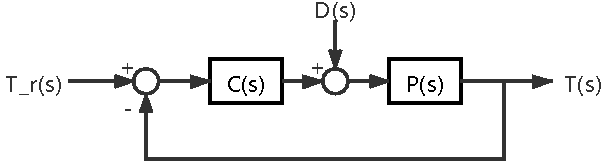
\includegraphics[width=13cm]{fig/block.pdf}
    \caption{Block diagram for the system with a PID controller}
    \label{fig:block}
    \end{figure}
  Finally, the transfer function for the system with the PID controller is formulated as
  \begin{equation}\label{equ:allsys}
  T(s)=\frac{C(s)P(s)}{1+C(s)P(s)}\cdot T_r(s) +\frac{P(s)}{1+C(s)P(s)}\cdot D(s),
  \end{equation}
  where $T_r(s)$ and $D(s)$ are the inputs for the system as a reference and disturbance. As for the numerical values for the other parameters in case study:
  \begin{itemize}
    \item Initial room temperature $T_0$ is $16\ ^\circ C$
    \item The reference temperature $T_r$ is changing between $16$ and $20\ ^\circ C$ every $5000$ seconds
    \item The total simulation period $T_f$ is $20,000$ seconds.
    \item The disturbance is a sinusoidal function as $2+0.5 \cdot \sin(\frac{t}{500})$.
    \item The initial values for the PID parameters are $K_p=K_i=K_d=0.5$
  \end{itemize}

  \subsubsection{System Simulation in Julia}
  The simulation for the system described in Equation~\eqref{equ:allsys} is realized using \verb|ControlSystem.jl| package in Julia~\cite{Carlson2016ControlSystemsjlA}. Firstly, the subsystem with input $T_r(s)$ in Equation~\eqref{equ:allsys} is implemented in function \verb|Tref(p)| following the flow chart in Figure~\ref{fig:system}. The simulation will take the values for PID as an input and output the time response of the system within the required time period.
    \begin{figure}[t]
    \centering
    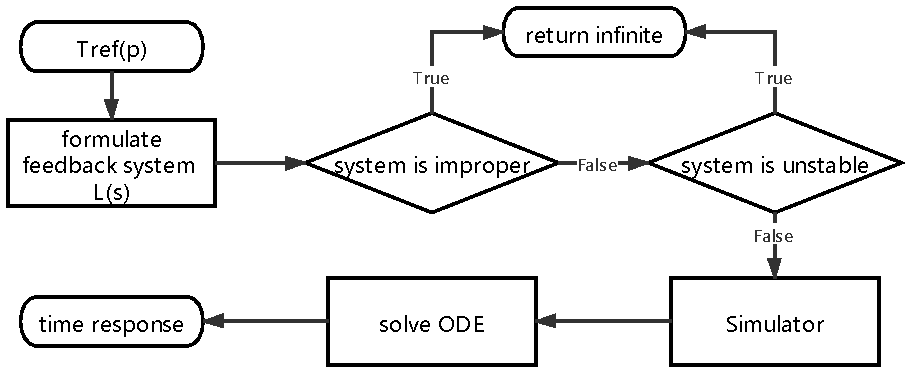
\includegraphics[width=13cm]{fig/system.pdf}
    \cprotect\caption{System simulation in Julia for \verb|Tref|}
    \label{fig:system}
    \end{figure}

  To explain, before the simulation, the transfer function for the feedback system should be proper (more poles than zeros) and stable so that the \verb|ControlSystem.jl| will not waste time solving an unstable system using some inappropriate PID arguments. Then, a simulator is used to translate the system with given input signal to ordinary differential equations (ODEs), which is a manner that can be solved by an ODE solver. Then, the function \verb|solve| will solve the ODEs with given initial condition $x_0$ within a time period \verb|tspan|. For the simulation of the system with a long time scale, the function \verb|solve| should be adapted to decrease the time for solving the ODEs~\cite{rackauckas2017differentialequations}. The arguments combination with their values (selected by the author) are as followed
  \begin{minted}[breaklines,escapeinside=||,mathescape=true, linenos, numbersep=3pt,frame=lines, gobble=2, fontsize=\small, framesep=2mm]{julia}
      sol   = solve(s, x0, tspan,maxiters=1e7,dtmin=0.001,reltol = 1e-1,force_dtmin=true)
      \end{minted}

  \begin{itemize}
    \item \verb|maxiters| adjusts the maximum number of iterations before stopping. The value needs to be increased to allow a long time scale simulation.
    \item \verb|dtmin| adjusts the minimum time step \verb|dt| for adaptive timestepping (only works for adaptive method). This value needs to be large so that the solver will not waste time calculating an excessive precise solution. Meanwhile, the \verb|force_dtmin| should be set as \verb|true|, which allows the solver to continue when encountering the minimum time step. Otherwise, the solving process will be terminated early once \verb|dt<dtmin|.
    \item \verb|reltol| adjusts the relative tolerance in adaptive timestepping. This value needs to be large as well for the same reason as above.
    \item The proper method should be carefully selected for different problems (i.e., stiff or non-stiff). In this project, the default solver of \verb|ControlSystem.jl| - \verb|Tsit5| (Tsitouras 5/4 Runge-Kutta method) are used to solve the ODEs. 
  \end{itemize}

  Then, the same procedure is repeated for the subsystem with input $D(s)$ with function \verb|Tdis(p)|. At last, the time responses obtained from two subsystems are added element-wise to get the time response for the entire system described in Equation~\eqref{equ:allsys}, which is the dynamic of the actual room temperature within $20,000$ seconds.

  \subsubsection*{Integrated absolute value}
  The time response obtained from the simulation above has the type of \verb|Vector{Float64}|. Therefore the IAE can be calculated using 
  \begin{minted}[breaklines,escapeinside=||,mathescape=true, linenos, numbersep=3pt, gobble=2, frame=lines, fontsize=\small, framesep=2mm]{julia}
  function IAE(p)
      f_DS(p)=mean(abs, ref .- (Tref(p) .+ Tdis(p)))  # IAE
      return [f_DS]
  end
    \end{minted}
  This function could also be fed into \verb|DirectSearch.jl| as an objective function with the PID parameters as an input.

  \subsubsection*{Maximum sensitivity}
  $S(s)$ in Equation~\eqref{equ:dist} can be evaluated using function \verb|bode| to get the magnitude for its frequency response. The output \verb|mag| has the type of \verb|Vector{Float64}|. Then, the largest value in this set is the maximum sensitivity.
  % \begin{minted}[breaklines,escapeinside=||,mathescape=true, linenos, numbersep=3pt, gobble=2, frame=lines, fontsize=\small, framesep=2mm]{julia}
  % function Disturbance(p)
  %     C     = Kpid(p[1], p[2], p[3])
  %     !isproper(P/(1 + P * C)) && return Inf
  %     L     = P/(1 + P * C) |> ss
  %     e,v=eigen(L.A) #ensure the system is stable
  %     any(>=(0), e) && return Inf

  %     mag, phase, w = bode(L)
  %     return maximum(abs.(mag[:,1,1]))
  % end
  %   \end{minted}
    Finally, the bi-objective problem for the building case is formulated as in List~\ref{lis:build}.
        \begin{listing}[ht]
      \begin{minted}[breaklines,escapeinside=||,mathescape=true, linenos, numbersep=3pt, gobble=2, fontsize=\small, framesep=2mm]{julia}
  function Building_bimads(p)
      IAE(p)=mean(abs, ref .- (Tref(p) .+ Tdis(p)))  # IAE
      sen(p)=Disturbance(p) # Maximum sensitivity
      return [IAE, sen]
  end
    \end{minted}
  \cprotect\caption{Bi-objective problem for building case}
  \label{lis:build}
  \end{listing}

  \subsection{Test Functions Set}
  The Julia and C++ packages for BiMADS will be tested on 20 bi-objective optimization problems selected from~\cite{zitzler2000comparison,davidor1994parallel,huband2006review,brockhoff2016using,deb2002scalable}. The comparison will be made regarding the running time and number function evaluation used to achieve the maximum hypervolume (accurate to two decimal places). The selected problems all have certain difficulties for finding the Pareto optimum front, such as:
  \begin{itemize}
  \item The multimodality problems have multiple minima, where the optimizer might become stuck in.
  \item The bias problems have more solutions that exist in some areas of objective space than in others, which affects the convergence speed toward the Pareto front.
  \item The geometries of the Pareto fronts can be convex, concave, discontinuous or even some combination of former (mixed front)~\cite{huband2006review}. Also, the solutions along the Pareto front can be non-uniform distributed, which means the densities of the points are different in different areas. Thus, the optimizer might waste time searching in the gaps or fail to find all regions of the Pareto front.
  \item The dimension of the variable is large, so is the search space. The optimizer will need more function evaluations to find a better point.
  \end{itemize}

  All the selected problems are presented in Table~\ref{tab:probs} with dimension $m$ and their main features. The mathematical expressions and the Pareto fonts for all the problems are detailed in Appendix~\ref{sec:front}, where $f_1(x)$ and $f_2(x)$ are the objective functions for all problems.

  \begin{table}[tbp]
    \centering
    \caption{Selected Problems with their dimensions and main features}
      \begin{tabular}{lcl|lcl}
      \toprule
  \textbf{Problems} & $\mathbf{m}$ & \textbf{Mian Features} & \textbf{Problems} & $\mathbf{m}$ & \textbf{Main Features}\\
      \hline    
      ZDT1~\cite{huband2006review} & 30 & convex & ZDT2~\cite{huband2006review} & 30 & concave \\
      ZDT3~\cite{huband2006review} & 30 & discontinuous & ZDT4~\cite{huband2006review} & 10 & multimodality\\
      ZDT6~\cite{huband2006review} & 10 & bias & F5.1~\cite{audet2008multiobjective} & 2 & convex \\
      F5.2~\cite{audet2008multiobjective} & 2 & concave & F5.3~\cite{audet2008multiobjective} & 2 & discontinuous \\
      F5.4~\cite{audet2008multiobjective} & 2 & bias & F5.5~\cite{audet2008multiobjective} & 2 & non-uniform \\  
      F1~\cite{brockhoff2016using} &5 & convex & DTLZ1~\cite{huband2006review} & 2 &  multimodality\\
      MOP2~\cite{huband2006review} & 4 & concave & MOP3~\cite{huband2006review} & 2 & convex \\
      MOP4~\cite{huband2006review} & 3& discontinuous & MOP6~\cite{huband2006review}&2& mixed front \\
      FES1~\cite{huband2006review} & 10 & mixed front & QV1~\cite{huband2006review}& 10 & concave\\
      OKA1~\cite{davidor1994parallel} &2  & bias & FAR1~\cite{huband2006review}& 2 & mixed front \\
      \bottomrule
      \end{tabular}%
    \label{tab:probs}%
  \end{table}%


\section{Result and Evaluation}\label{sec:reseva}
This section provides the results of the building case study with evaluation. Then the test results of \verb|Direct-| \verb|Search.jl| and \verb|NOMAD| on the same bi-objective problem set are presented and compared. At last, a short result for the unit test is shown with the measurement of the code coverage.
\subsection{Building case study}
\subsubsection{Result}
The bi-objective problem is formulated as in List~\ref{lis:build} with initial condition $p=[0.5,0.5,0.5]$. The iteration limit is set to 100 because the simulation of the long time period system is quite time-consuming. The Pareto front is finally obtained as shown in Figure~\ref{fig:pareto1}, where the minimum value for IAE and maximum sensitivity is 1.74 and 0.00414, respectively. However, the corresponding IAE for the minimum sensitivity is 17.86, which is too large and ignored. Thus, the upper left part is zoomed in as in Figure~\ref{fig:pareto2}. The numerical costs for these six points with their PID parameters are shown in Table~\ref{tab:value_build}. Also, the result of the initial condition and the ignored point are also point 0 and 7 in Table~\ref{tab:value_build}.

 \begin{figure}[t]
  \centering
  \subfigure[Pareto front]{ \label{fig:pareto1}
  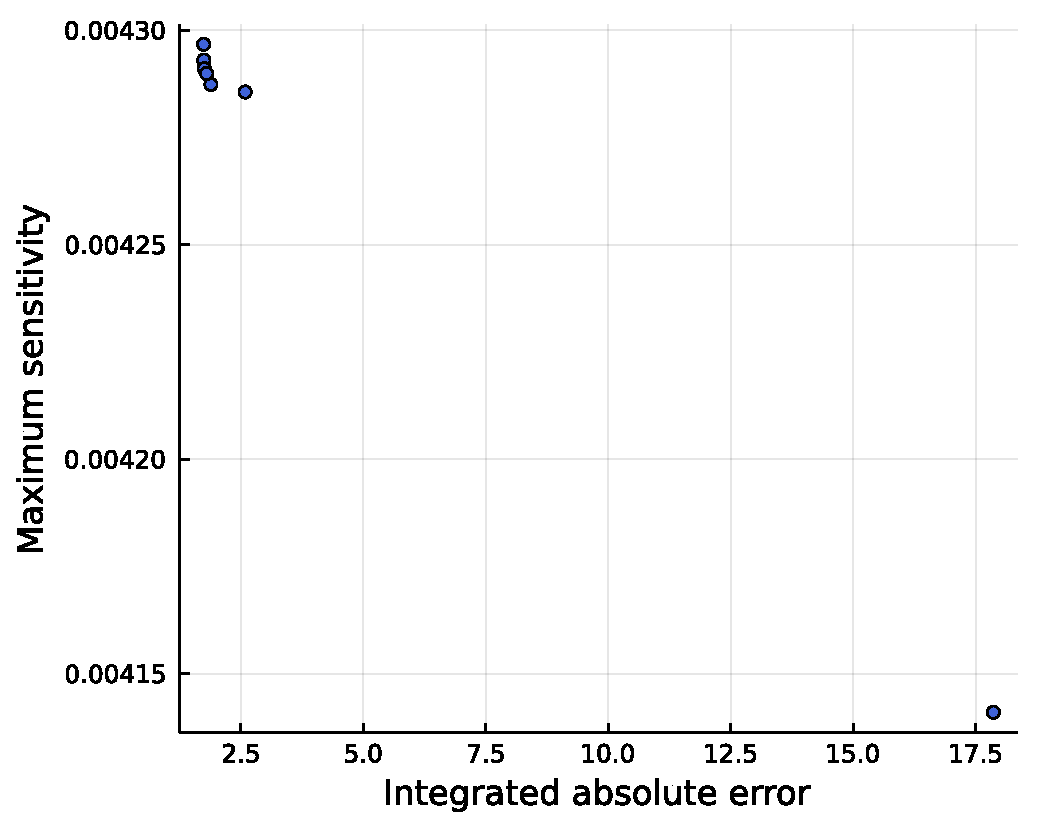
\includegraphics[width=8cm]{fig/pareto1.pdf}}
    \subfigure[Pareto front (zoom in)]{ \label{fig:pareto2}
  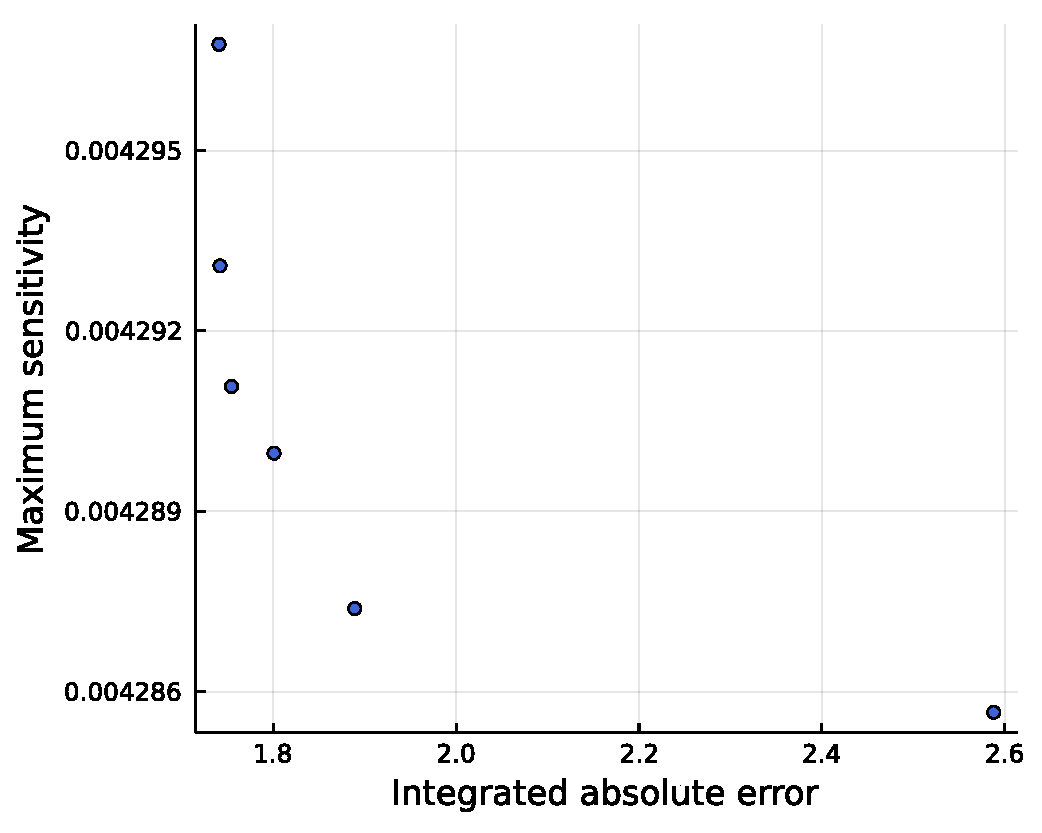
\includegraphics[width=8cm]{fig/pareto2.pdf}}
  \caption{Pareto front for the building case study}
  \label{fig:pareto_build}
  \end{figure}

\begin{table}[t]
  \centering
  \caption{Numerical costs and PID parameters}
    \begin{tabular}{c|ccc|c|ccc}
    \toprule
    \textbf{point} & \textbf{IAE} & \textbf{Max sensitivity} & \textbf{PID ($K_p,K_i,K_d$)} & \textbf{point} & \textbf{IAE} & \textbf{Max sensitivity} & \textbf{PID ($K_p,K_i,K_d$)} \\
    \hline
    0 & 6.071 & 0.005578 &  0.50, 0.50, 0.50 & 1 & 1.740 & 0.004297 & -0.75, 0.62, 0.08 \\
    2 & 1.741 & 0.004293 & -0.55, 0.62, 0.08 & 3 & 1.754 & 0.004291 & -0.45, 0.67, 0.10 \\
    4 & 1.800 & 0.004289 & -0.25, 0.47, 0.17 & 5 & 1.889 & 0.004287 & -0.25, 0.47, 0.10 \\
    6 & 2.588 & 0.004285 & -0.18, 0.47, 0.15 & 7 & 17.86 & 0.004142 &  7.96, 0.16, 10.99 \\
    \bottomrule
    \end{tabular}%
  \label{tab:value_build}%
\end{table}%

  The Pareto font in Figure~\ref{fig:pareto2} shows that although the points at two ends have small values in terms of one criterion but large values for the other. Thus, the middle points are preferable for the building case. The time responses for point 4 and 5 are shown in Figure~\ref{fig:resp_build}, which have comparatively small IAE and sensitivity at the same time.
   \begin{figure}[t]
  \centering
  \subfigure[Time response for point 4]{ \label{fig:best}
  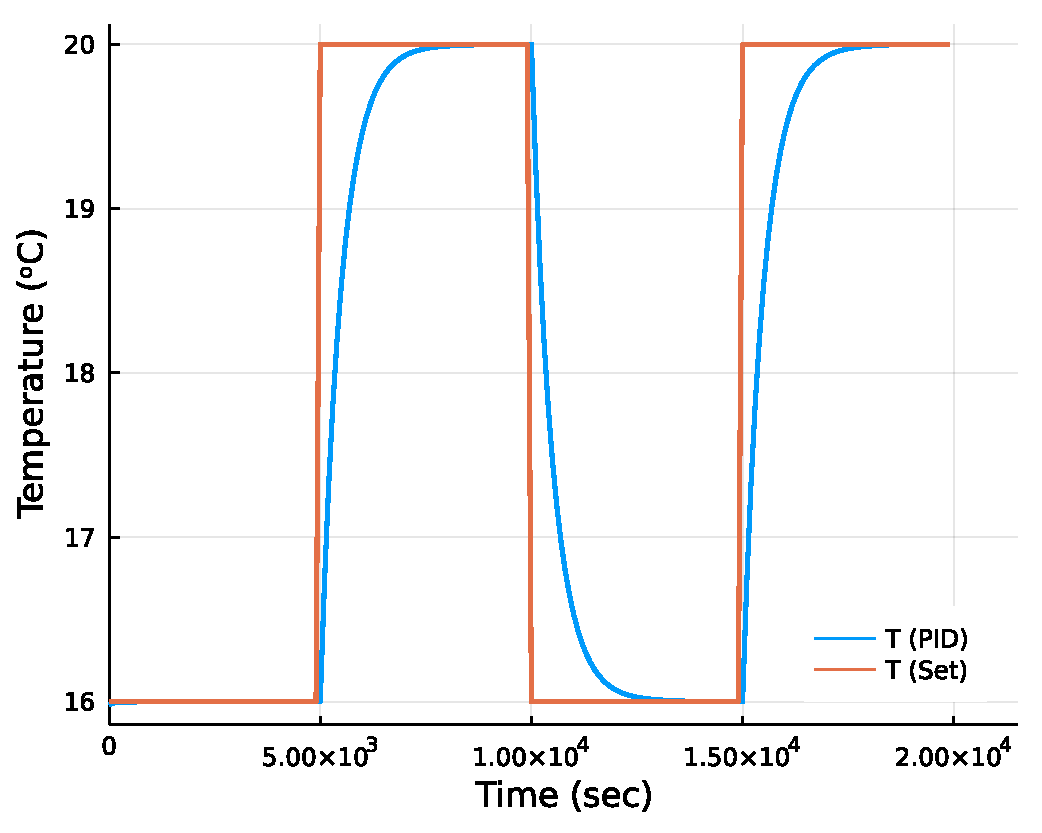
\includegraphics[width=8cm]{fig/best.pdf}}
    \subfigure[Time response for point 5]{ \label{fig:med}
  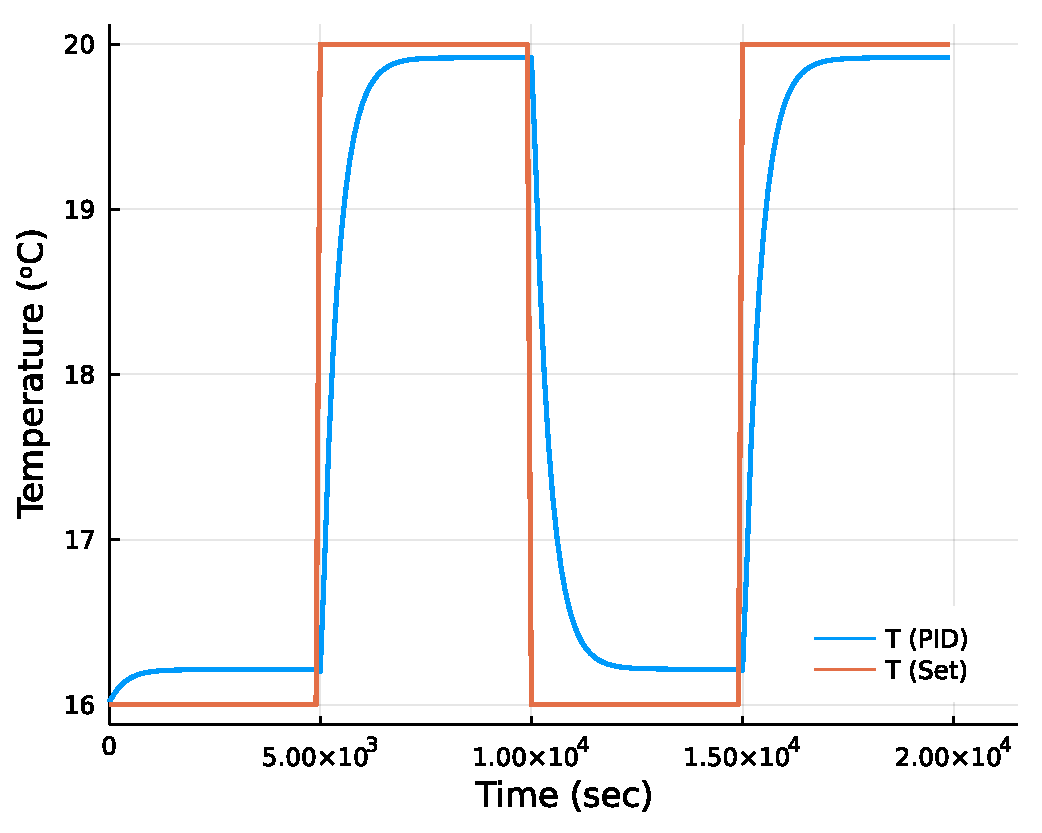
\includegraphics[width=8cm]{fig/medium.pdf}}
  \caption{Time responses for point 4 and 5}
  \label{fig:resp_build}
  \end{figure}

\subsubsection{Evaluation}
The results show that the actual room temperature could follow the pre-set value and resist the external disturbance at the same time. The parameter for point 4 (Figure~\ref{fig:best}) has a smaller IAE, hence the temperature follows the setpoint better but is more sensitive to the disturbance. In contrast, the parameter for point 4 (Figure~\ref{fig:med}) enables the system to be more robust to the disturbance but has a large IAE as a trade-off. Due to the small maximum sensitivity for all the Pareto solutions, the effect from disturbance is not obvious in both cases.

Also, the points are non-uniformly distributed on the Pareto front, where most of the solutions have small IAE but large sensitivity. The reason is that for most PID parameters that provide small sensitivity, the corresponding IAE is extremely large. Therefore, most of these points will be dominated by the lower right point in Figure~\ref{fig:pareto1}, which is the solution with the smallest sensitivity.

Lastly, learning from the experience of solving this bi-objective problem, several general suggestions might be helpful to solve other problems:
\begin{enumerate}
  \item If it takes a much longer time to get the cost for one of the objective functions, users are suggested to implement single-objective optimization first for this function to get the optimum solution. Then, the solution could be set as the initial point for the bi-objective optimization, which may save the time used for the BiMADS initialization stage.
  \item If one of the objectives is more important than the other, the users are suggested to run the bi-objective optimization only for a few BiMADS iterations first to see the Pareto front. Then, the users could narrow the search space by setting the constraints for the objective functions so that the BiMADS will not waste time searching in a useless space. 

  For example, IAE is more important than sensitivity because the sensitivity is already a small value for the building case. Without the constraints, BiMADS will waste time filling the large gap in Figure~\ref{fig:pareto1}, which is unnecessary due to the very large IAE. After focusing on a narrow space such as in Figure~\ref{fig:pareto2}, more valuable points with reasonable IAE and comparatively small sensitivity can be found.
\end{enumerate}


\subsection{Bi-objective problem set}
\subsubsection{Result}
To ensure \verb|NOMAD| and \verb|DirectSearch.jl| run the optimization in a similar way, some of the settings must be the same. For example:
\begin{itemize}
  \item The initial point, function evaluation budgets for each BiMADS iteration should be the same.
  \item Turn off the Nelder Mead Search and Speculative search in \verb|NOMAD| because \verb|DirectSearch.jl| does not have these two algorithms for search step.
\end{itemize}

  As a result, all the Pareto fronts generated by \verb|DirectSearch.jl| are shown in Appendix~\ref{sec:front}. Figure~\ref{fig:far1_eg} shows the Pareto fronts of FAR1 generated by two packages as an example. Most of the results from \verb|NOMAD| are similar to \verb|DirectSearch.jl|, hence they will not be presented individually. The running time, the number of function evaluations and the number of total generated solutions for both packages are shown in Table~\ref{tab:res_set}. All the results are the mean value from 10 instances because BiMADS is a non-deterministic algorithm. In addition, \verb|NOMAD| struggles to optimize several complex problems and cannot provide the Pareto fronts with enough hypervolume, even after a long time. These problems will be labelled with $*$ and the listed values are for their longest running time.

   \begin{figure}[t]
  \centering\cprotect
  \subfigure[Result from \verb|DirectSearch.jl|]{ \label{fig:ds}
  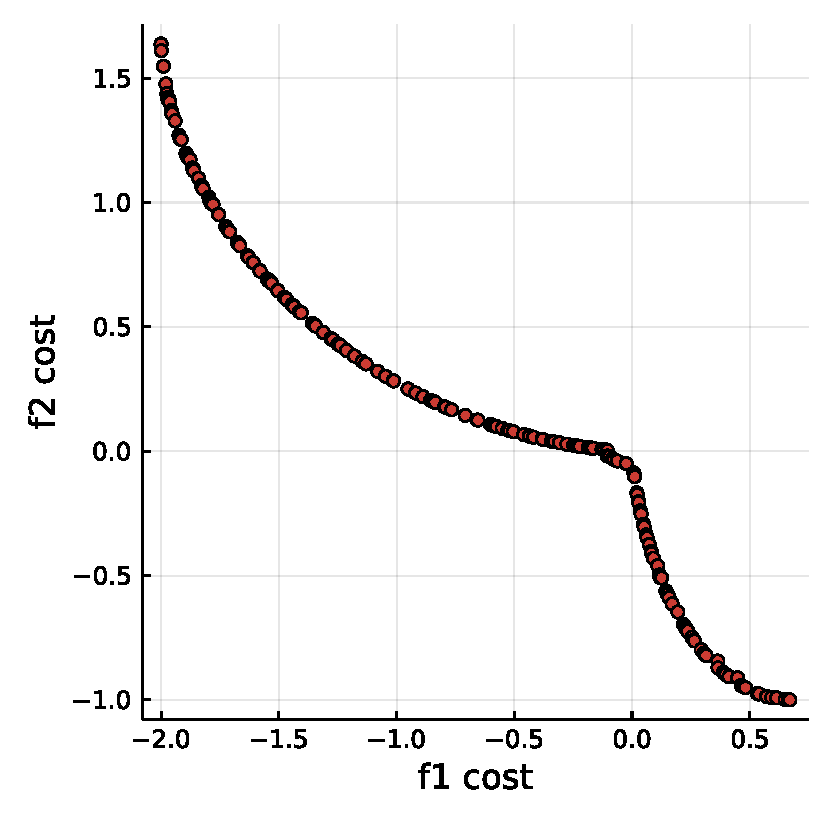
\includegraphics[width=8cm]{fig/FAR1.pdf}}
   \cprotect \subfigure[Result from \verb|NOMAD|]{ \label{fig:nomad}
  \includegraphics[width=8cm]{fig/FAR1_nomad.pdf}}
  \caption{Pareto fronts for FAR1, which is the mixed front with both convex and concave elements}
  \label{fig:far1_eg}
  \end{figure}


\begin{table}[]
  \centering
  \caption{Summary of the test for both packages}
    \begin{tabular}{c|cc|cc|cc}
    \toprule
     & \multicolumn{2}{c|}{\textbf{Running time (sec)}} & \multicolumn{2}{c|}{\textbf{Function evaluations}} & \multicolumn{2}{c}{\textbf{Total points}} \\
     Problem & DirectSearch & NOMAD & DirectSearch & NOMAD & DirectSearch & NOMAD\\
    \hline
    ZDT1$^*$~\cite{huband2006review} & 5.38 & 480 & 82099 &4524 &355 & 52\\
    ZDT2$^*$~\cite{huband2006review} & 6.63 & 511 & 34795  & 5323 & 423 & 66 \\
    ZDT3$^*$~\cite{huband2006review} & 7.22 & 309 & 94106 & 3320 & 695 & 32 \\
    ZDT4~\cite{huband2006review} & 0.75 & 394 & 86819 & 4198 & 879 & 26 \\
    ZDT6~\cite{huband2006review} & 3.58 & 420 & 63502 & 3897 & 820 & 119 \\
    F5.1~\cite{audet2008multiobjective} & 1.82 & 24 & 18398 & 607 & 923 & 147 \\
    F5.2~\cite{audet2008multiobjective} & 1.54 & 23 & 18828 & 602 & 873 & 132  \\
    F5.3~\cite{audet2008multiobjective} & 1.92 & 48 & 19672 & 1207& 809 & 201 \\
    F5.4~\cite{audet2008multiobjective} & 0.37 & 18 & 5880 & 632 & 164 & 110 \\
    F5.5~\cite{audet2008multiobjective} & 0.39 & 15 & 6392  & 617 & 373 & 107 \\
    F1~\cite{brockhoff2016using} & 0.26 & 17 & 11291 & 609 & 287 & 113 \\
    DTLZ1~\cite{huband2006review} & 1.90 & 22 & 21694 & 1205 & 995 & 115 \\
    MOP2~\cite{huband2006review} & 0.21 & 32 & 5116 & 607 & 202 & 135 \\
    MOP3~\cite{huband2006review} & 7.02 & 92 & 79591 & 1728 & 1037 & 587 \\
    MOP4~\cite{huband2006review} & 1.19 & 123 & 28493 & 2391 & 302 & 211 \\
    MOP6~\cite{huband2006review} & 0.41 & 45 & 8913 & 870 & 387 & 175 \\
    FES1~\cite{huband2006review} & 0.85 & 102 & 23297 & 1654 & 302 & 105 \\
    QV1~\cite{huband2006review} & 0.50 & 43 & 5350 & 625 & 221 & 95 \\
    OKA1~\cite{davidor1994parallel} & 4.8 & 89 & 42789 & 5168 & 151 & 44 \\
    FAR1~\cite{huband2006review} & 1.03 & 34 & 4902 & 626 & 401 & 214 \\
    \bottomrule
    \end{tabular}%
  \label{tab:res_set}%
\end{table}%

According to Table~\ref{tab:res_set}, the performance profiles are plotted in Figure~\ref{fig:perform} by \verb|BenchmarkProfiles.jl| for the comparison of two packages, which illustrates the proportion of the problems that the solver can solve within a factor $\tau$ of the best solver.

   \begin{figure}[t]
  \centering
  \subfigure[For running time]{ \label{fig:time}
  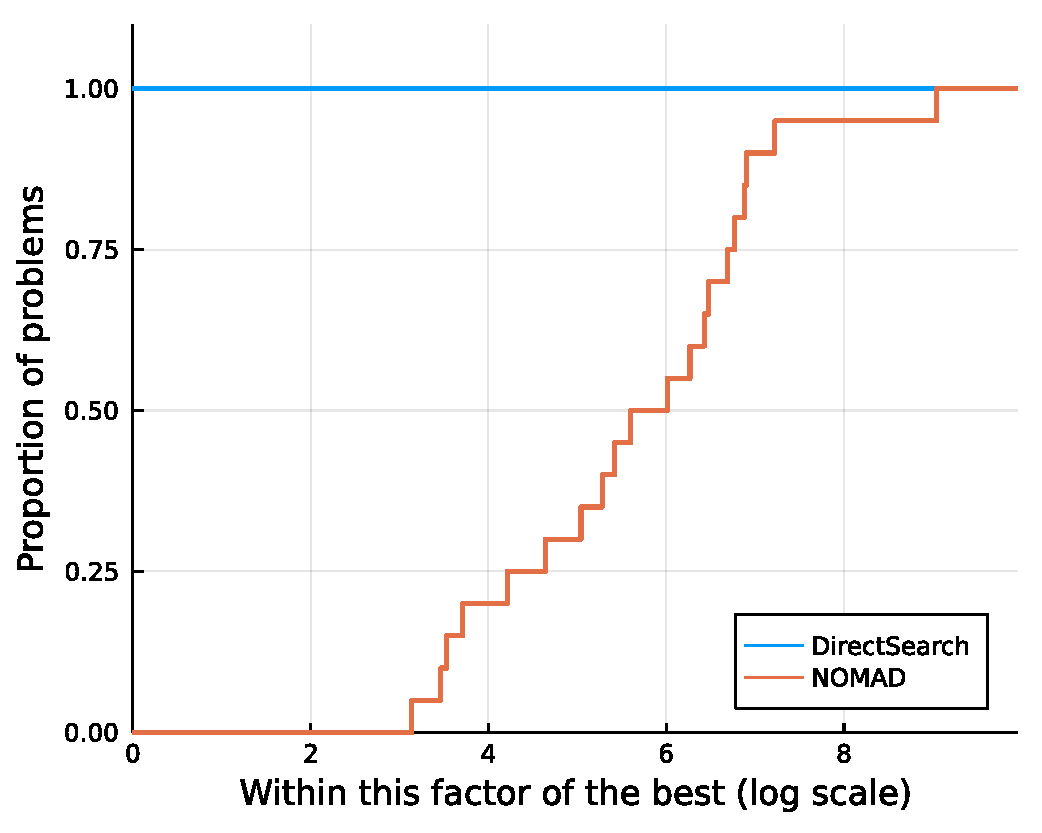
\includegraphics[width=8cm]{fig/time_perfom.pdf}}
    \subfigure[For function evaluation]{ \label{fig:eval}
  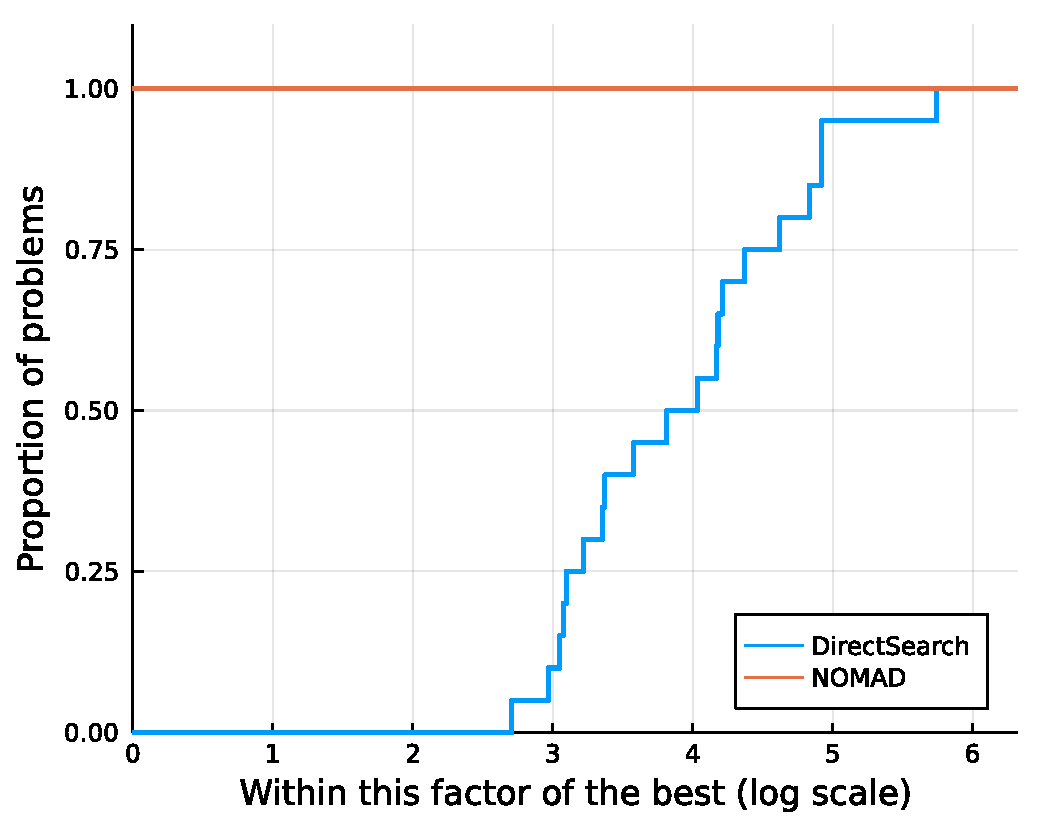
\includegraphics[width=8cm]{fig/bb_perfom.pdf}}
  \caption{Performance profiles}
  \label{fig:perform}
  \end{figure}

\subsubsection{Evaluation}
The package \verb|DirectSearch.jl| could solve all the problems within a short time, while \verb|NOMAD| requires an extremely long time to solve three of them. A common feature for these three problems is that they all have large dimensions of variable space ($m=30$). Also, from the performance profile, in terms of the running time (Figure~\ref{fig:time}), \verb|NOMAD| always requires much more time than \verb|DirectSearch.jl| to achieve the same hypervolume. In contrast, the number of function evaluations spent by \verb|DirectSearch.jl| is always much more than \verb|NOMAD| (Figure~\ref{fig:eval}). Due to a large number of function evaluations, the number of generated points on the Pareto front is also larger than in \verb|NOMAD|.

From the evaluations above, several features for two packages can be concluded as:
\begin{enumerate}
  \item Comparing with \verb|NOMAD|, \verb|DirectSearch.jl| tends to solve the problems by evaluating much more trial points in all directions to find a new Pareto solution. Benefiting from the fast speed of Julia, \verb|DirectSearch.jl| could evaluate more points while maintaining a short total running time. 
  \item As for \verb|NOMAD|, each function evaluation takes a much longer time, especially for the high dimensional problem, which needs the evaluations on more trial points to find a better solution. Hence, the \verb|NOMAD| first utilizes some searching algorithms such as Nelder Mead Search for the search step in MADS (not in this project). This step will search around all the space to find the better solution instead of only focusing on the current incumbent solution. Furthermore, \verb|NOMAD| chooses the trail points in a more clever way so that it can achieve the optimum solution by only evaluating a limited number of points.
  \item The number of the points generated by \verb|DirectSearch.jl| is much larger than in \verb|NOMAD|, which means users have more options when selecting the Pareto solutions. 
  \item If the obtained Pareto front is not as expected (i.e., too few points), the function evaluation limit for each BiMADS iteration should be increased first instead of only increasing the BiMADS iterations. The reason is that for some difficult problems (i.e., non-uniform Pareto front), the evaluation budget for each iteration is crucial to evaluate enough trial points for reformulated function $\phi_r$. Hence, more points could be generated in a single BiMADS iteration.
\end{enumerate}

In summary, \verb|DirectSearch.jl| relies on a large number of function evaluations and has a fast evaluating speed for a single trail point. Therefore, it is suitable for problems with any dimensions. However, some problems naturally take a long time to return their costs in each evaluation (i.e., simulation of long-period systems). These problems are more suitable for \verb|NOMAD| because it could find the Pareto solutions with a limited number of function evaluations.

\subsection{Unit test}
The result of the unit test is shown in Figure~\ref{fig:unit_test}, which shows that all the test functions designed for BiMADS have passed the unit test. The Julia package \verb|Coverage.jl| is used to track each line of the code and count how many times does it run. This is called a code coverage test, which reveals the parts of the code that is not tested yet and may have bugs. After applying this test, the code coverage for the designed unit test is $100\%$ so that all the code implementations for BiMADS have been tested.

    \begin{figure}[t]
    \centering
    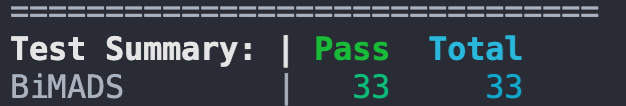
\includegraphics[width=8cm]{fig/unit_test.png}
    \caption{Result of the unit test}
    \label{fig:unit_test}
    \end{figure}
% ds生成的点多
% 某些问题需要每次iteraiotn多点
%DS 可以做更多eval所以能找到更多点,对于dimension大的问题,需要更多的trial points而NOMAD提供的点太少,所以找不到解
% NOMAD适合于dim小,而且单次访问时间高的问题,ds适合任何dim,但是不适合单次时间高的问题
% Unit test and Code Coverage

\section{Conclusions and Future Work}
% stalling
% Bimads 结构,吧dsproblem单独领出来做abstracproblem
% 加 Bimas iteration limit, 每一次iteration的eval number
% multi-polling?
\subsection{Conclusions}
  This project extended the Julia optimization package \verb|DirectSearch.jl| with the BiMADS algorithm, which enables the package to solve bi-objective problems and get the Pareto optimum set. Apart from the original algorithm, several new stopping conditions are added to improve the flexibility of the package. The developed package was first tested on a real-life PID design problem, which aims to control the room temperature and resist the effect from outside disturbance. Then, the performance of BiMADS in \verb|DirectSearch.jl| was compared with a state-of-art bi-objective optimization solver \verb|NOMAD| on a test set. The implementation of BiMADS in \verb|DirectSearch.jl| is outstanding in terms of running time and provides more flexibility for the users.

 \subsection{Future work}
\begin{enumerate}
  \item The hypervolume indicator only support bi-objective optimization and there is no advanced algorithm applied for the calculation. In the future, the indicator should be extended to multi-dimension to support multi-objective optimization. Also, a new algorithm should be introduced to improve the speed because the calculations for high dimensional hypervolume is time-consuming.
  \item One of the drawbacks for BiMADS is that the algorithm may stall in some iteration, which wastes the function evaluation budget searching in a narrow space. Inspired from DMulti-MADS~\cite{bigeon2021dmulti}, the optimization of the reformulated function $\phi_r$ needs to be adapted: 1) To avoid getting stuck in a narrow space, the search step for MADS should not be skipped. 2) Multi-polling may be used to implement poll step on multiple trail points to increase the searching space.
  \item As for the code in Julia, multiple dispatch can be used on formulating the bi-objective problem. A new type with the same namespace \verb|DSProblem| can be designed, which inherits from \verb|AbstractProblem|. To distinguish from old \verb|DSProblem|, the new type will have several new input arguments such as total BiMADS iteration limit and hypervolume limit. The new type could simplify the code structure, improve efficiency and benefit future development.
\end{enumerate}

\newpage
{\small
\begin{spacing}{1.0}
\bibliographystyle{IEEEtran}
\bibliography{reference}
\addcontentsline{toc}{section}{Reference}
\end{spacing}
}

\newpage
\section{Appendix}
\subsection{User Guide}
  The \href{https://imperialcollegelondon.github.io/DirectSearch.jl/dev/}{\textcolor{blue}{documentation}} for the current public version of \verb|DirectSearch.jl| explains how to optimize a single-objective problem with MADS in detail. However, the code implemented in this project has not been released so far. Therefore, a simple instruction on how to optimize a bi-objective problem MOP4 (see Section~\ref{sec:mop4}) is shown below:
  \begin{enumerate}
  \item Objective functions should be first declared as a function:
    \begin{minted}[breaklines,escapeinside=||,mathescape=true, linenos, numbersep=3pt, gobble=2, frame=lines, fontsize=\small, framesep=2mm]{julia}
    function obj(x)
      f1(x) = sum(-10 * exp.(-0.2 * sqrt.(x[1:2].^2 + x[2:3].^2)))
      f2(x) = sum(abs.(x).^0.8 + 5 * sin.(x.^3))
        return [f1,f2]
    end
    \end{minted}
    \item The \verb|DSProblem| is then formulated with initial condition as
      \begin{minted}[breaklines,escapeinside=||,mathescape=true, linenos, numbersep=3pt, gobble=2, frame=lines, fontsize=\small, framesep=2mm]{julia}
    p = DSProblem(3; objective=obj,initial_point=[0., 0., 0.])
    \end{minted}
    \item The parameters such as iteration limit and function evaluation limit are set in the same way as shown in the public documentation.
    \item The \verb|key interrupt| stopping condition are activated by default. The other two new stopping conditions can be set as
        \begin{minted}[breaklines,escapeinside=||,mathescape=true, linenos, numbersep=3pt, gobble=2, frame=lines, fontsize=\small, framesep=2mm]{julia}
   AddStoppingCondition(p, HypervolumeStoppingCondition(1.3))#hypervolume limit
   AddStoppingCondition(p, RuntimeStoppingCondition(2.0))#run time limit
    \end{minted}
    \item Run the optimization using
        \begin{minted}[breaklines,escapeinside=||,mathescape=true, linenos, numbersep=3pt, gobble=2, frame=lines, fontsize=\small, framesep=2mm]{julia}
    result=Optimize!(p)
    \end{minted}
    \verb|result| is of the type \verb|Vector{B_points}| and stores all the Pareto solutions with their costs in terms of \verb|f1| and \verb|f2|. The costs can be used for plotting the Pareto front as
        \begin{minted}[breaklines,escapeinside=||,mathescape=true, linenos, numbersep=3pt, gobble=2, frame=lines, fontsize=\small, framesep=2mm]{julia}
        fig=plot_Bpoint(result)
    \end{minted}
    Based on the Pareto front, the users can select the solutions they prefer.
  \end{enumerate}


\newpage
\subsection{Bi-objective Problem set with Pareto fronts}\label{sec:front}
  \subsubsection{ZDT1~\cite{huband2006review}}
  \textbf{Dimension of variables: }$m=30$

  \noindent\textbf{Problem Statement: }
  \begin{equation}
  \begin{aligned}
  f_{1}\left(x_{1}\right) & =x_{1} \\
  g\left(x_{2}, \ldots, x_{m}\right) & =1+9 \cdot \sum_{i=2}^{m} x_{i} /(m-1) \\
  h\left(f_{1}, g\right) & =1-\sqrt{f_{1} / g}\\
  f_2(x_{1}, \ldots, x_{m})&=g\cdot h
  \end{aligned}
  \end{equation}
  \noindent\textbf{Constraints: } $x_{1}, \ldots, x_{m}\in [0,1]$\\
  \noindent\textbf{Features: }Convex, Large dimension\\
  \noindent\textbf{Hypervolume: } 1.44\\
  \noindent\textbf{Pareto front}
      \begin{figure}[H]
      \centering
      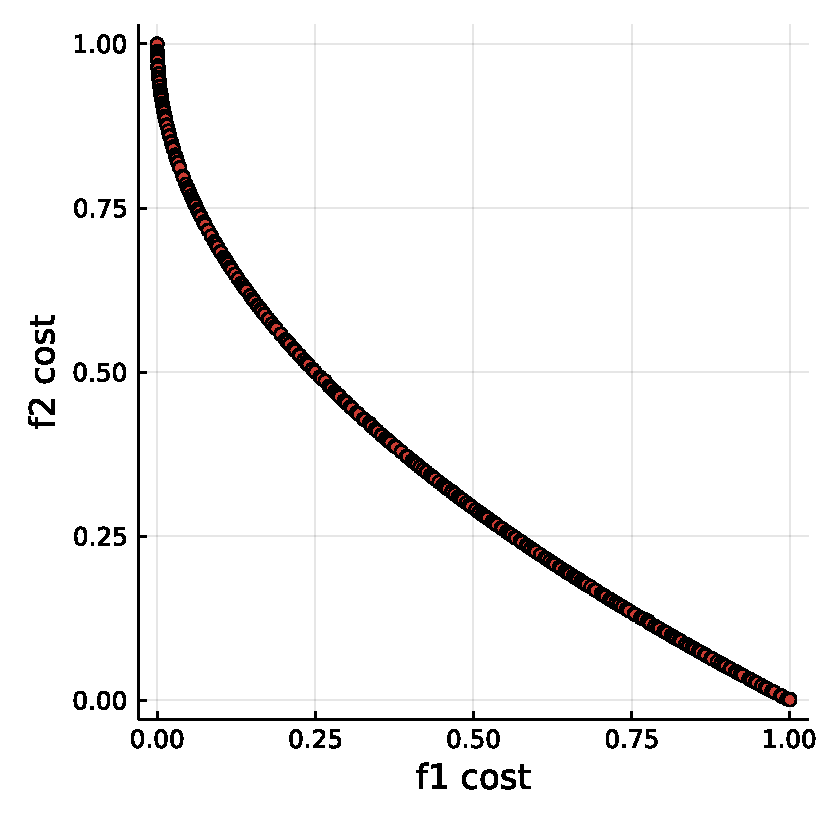
\includegraphics[width=12cm]{fig/cvx1.pdf}
      \cprotect\caption{Pareto front for ZDT1}
      \label{fig:ZDT1}
      \end{figure}

   \subsubsection{ZDT2~\cite{huband2006review}}
   \textbf{Dimension of variables: }$m=30$

  \noindent\textbf{Problem Statement: }
  \begin{equation}
  \begin{aligned}
  f_{1}\left(x_{1}\right) &=x_{1} \\
  g\left(x_{2}, \ldots, x_{m}\right) &=1+9 \cdot \sum_{i=2}^{m} x_{i} /(m-1) \\
  h\left(f_{1}, g\right) &=1-\sqrt{f_{1} / g}-\left(f_{1} / g\right) \sin \left(10 \pi f_{1}\right)\\
  f_2(x_{1}, \ldots, x_{m})&=g\cdot h
  \end{aligned}
  \end{equation}
  \noindent\textbf{Constraints: } $x_{1}, \ldots, x_{m}\in [0,1]$\\
  \noindent\textbf{Features: }Concave, Large dimension\\
  \noindent\textbf{Hypervolume: } 0.90\\
  \noindent\textbf{Pareto front}
      \begin{figure}[H]
      \centering
      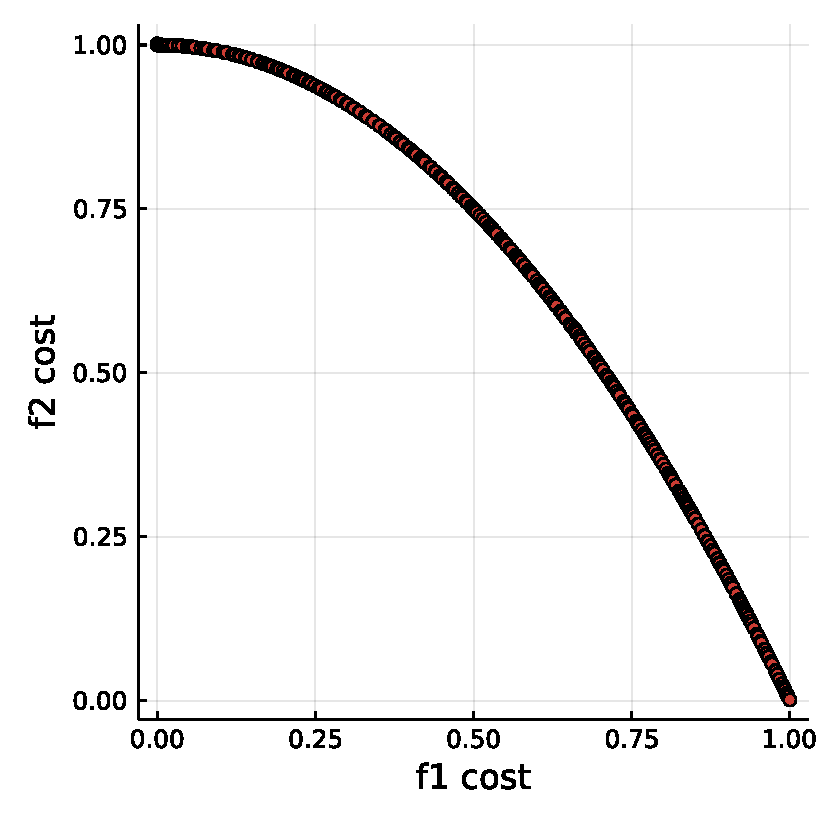
\includegraphics[width=12cm]{fig/ncvx1.pdf}
      \cprotect\caption{Pareto front for ZDT2}
      \label{fig:ZDT2}
      \end{figure}
   \subsubsection{ZDT3~\cite{huband2006review}}
  \textbf{Dimension of variables: }$m=30$

  \noindent\textbf{Problem Statement: }
  \begin{equation}
  \begin{aligned}
  f_{1}\left(x_{1}\right) &=x_{1} \\
  g\left(x_{2}, \ldots, x_{m}\right) &=1+9 \cdot \sum_{i=2}^{m} x_{i} /(m-1) \\
  h\left(f_{1}, g\right) &=1-\sqrt{f_{1} / g}-\left(f_{1} / g\right) \sin \left(10 \pi f_{1}\right)\\
  f_2(x_{1}, \ldots, x_{m})&=g\cdot h
  \end{aligned}
  \end{equation}
  \noindent\textbf{Constraints: } $x_{1}, \ldots, x_{m}\in [0,1]$\\
  \noindent\textbf{Features: } Discontinuous, Convex, Large dimension\\
  \noindent\textbf{Hypervolume: } 1.17\\
  \noindent\textbf{Pareto front}
      \begin{figure}[H]
      \centering
      \includegraphics[width=12cm]{fig/dt1.pdf}
      \cprotect\caption{Pareto front for ZDT3}
      \label{fig:ZDT3}
      \end{figure}
    \subsubsection{ZDT4~\cite{huband2006review}}
   \textbf{Dimension of variables: }$m=10$

  \noindent\textbf{Problem Statement: }
  \begin{equation}
  \begin{aligned}
  f_{1}\left(x_{1}\right) & =x_{1} \\
  g\left(x_{2}, \ldots, x_{m}\right) & =1+10(m-1)+\sum_{i=2}^{m}\left(x_{i}^{2}-10 \cos \left(4 \pi x_{i}\right)\right) \\
  h\left(f_{1}, g\right) & =1-\sqrt{f_{1} / g}\\
  f_2(x_{1}, \ldots, x_{m})&=g\cdot h
  \end{aligned}
  \end{equation}
  \noindent\textbf{Constraints: } $x_{1} \in[0,1]$, and $x_{2}, \ldots, x_{m} \in[-5,5]$\\
  \noindent\textbf{Features: } Multimodality\\
  \noindent\textbf{Hypervolume: } 1.91\\
  \noindent\textbf{Pareto front}
      \begin{figure}[H]
      \centering
      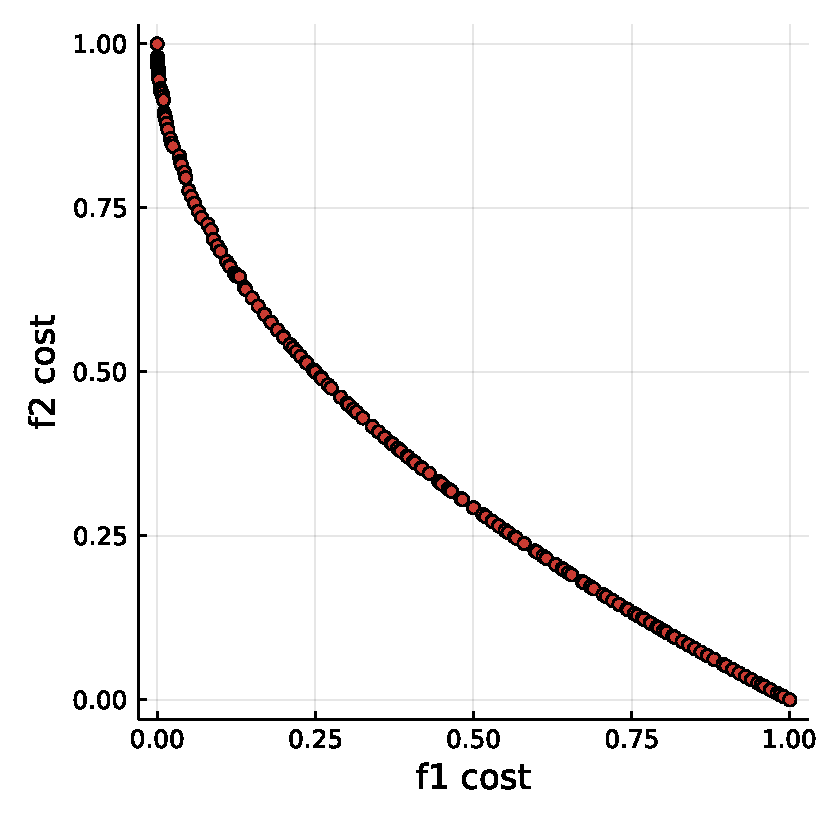
\includegraphics[width=12cm]{fig/mmod.pdf}
      \cprotect\caption{Pareto front for ZDT4}
      % \label{fig:ZDT1}
      \end{figure}

   
   \subsubsection{ZDT6~\cite{huband2006review}}
    \textbf{Dimension of variables: }$m=10$

  \noindent\textbf{Problem Statement: }
  \begin{equation}
  \begin{aligned}
  f_{1}\left(x_{1}\right) & =1-\exp \left(-4 x_{1}\right) \sin ^{6}\left(6 \pi x_{1}\right) \\
  g\left(x_{2}, \ldots, x_{m}\right) & =1+9 \cdot\left(\left(\sum_{i=2}^{m} x_{i}\right) /(m-1)\right)^{0.25} \\
  h\left(f_{1}, g\right) & =1-\left(f_{1} / g\right)^{2}\\
  f_2(x_{1}, \ldots, x_{m})&=g\cdot h
  \end{aligned}
  \end{equation}
  \noindent\textbf{Constraints: } $x_{1}, \ldots, x_{m} \in[0,1]$\\
  \noindent\textbf{Features: } Bias: non-uniform search space. \\
  \noindent Non-uniform: density of the solutions is lowest near the Pareto front.\\
  \noindent\textbf{Hypervolume: } 1.17\\
  \noindent\textbf{Pareto front}
      \begin{figure}[H]
      \centering
      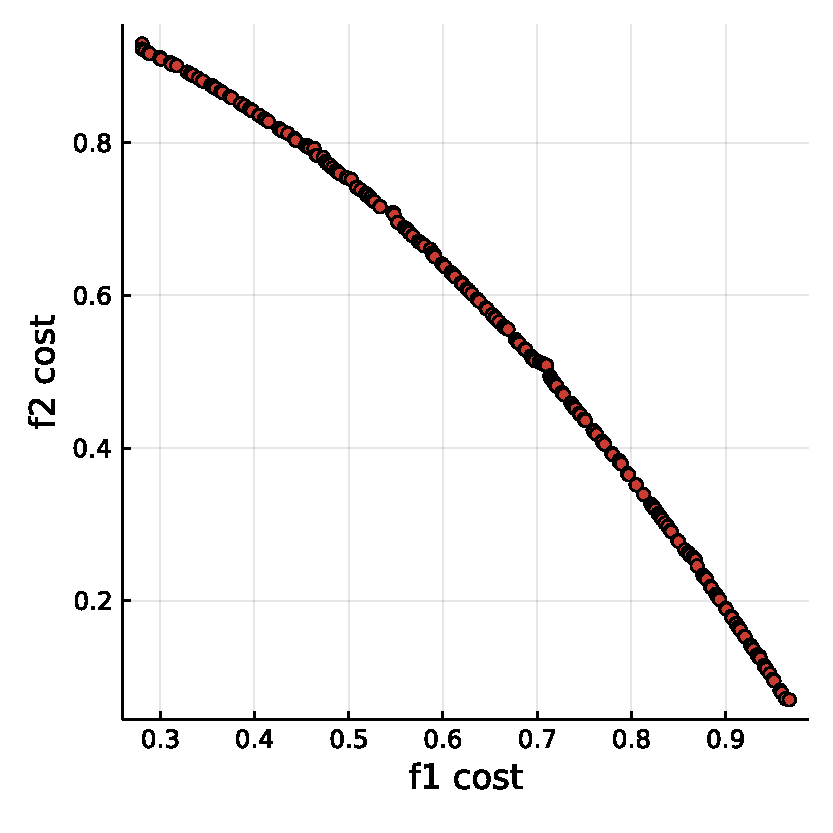
\includegraphics[width=12cm]{fig/nuni1.pdf}
      \cprotect\caption{Pareto front for ZDT6}
      % \label{fig:ZDT1}
      \end{figure}


   \subsubsection{F5.1~\cite{audet2008multiobjective}}
     \textbf{Dimension of variables: }$m=2$\\
  \noindent\textbf{Problem Statement: }
  \begin{equation}
  \begin{aligned}
  f_1(x_1) &= 4x_1 \\
  g\left(x_{2}\right)&= \begin{cases}4-3 \exp \left(-(\frac{x_{2}-0.2}{0.02})^{2}\right) & \text { if } 0 \leq x_{2} \leq 0.4 \\ 4-2 \exp \left(-(\frac{x_{2}-0.7}{0.2})^{2}\right) & \text { if } 0.4 \leq x_{2} \leq 1\end{cases}\\
  h\left(f_{1}, g\right)&= \begin{cases}1 -\left(\frac{f_{1}}{g}\right)^{0.25} & \text { if } f_{1} \leq g \\ 0 & \text { otherwise }\end{cases}\\
  f_2(x_{1}, x_{2})&=g\cdot h
  \end{aligned}
  \end{equation}
  \noindent\textbf{Constraints: } $x_{1}, x_{2} \in[0,1]$\\
  \noindent\textbf{Features: } Convex\\
  \noindent\textbf{Hypervolume: } 1.66\\
  \noindent\textbf{Pareto front}
      \begin{figure}[H]
      \centering
      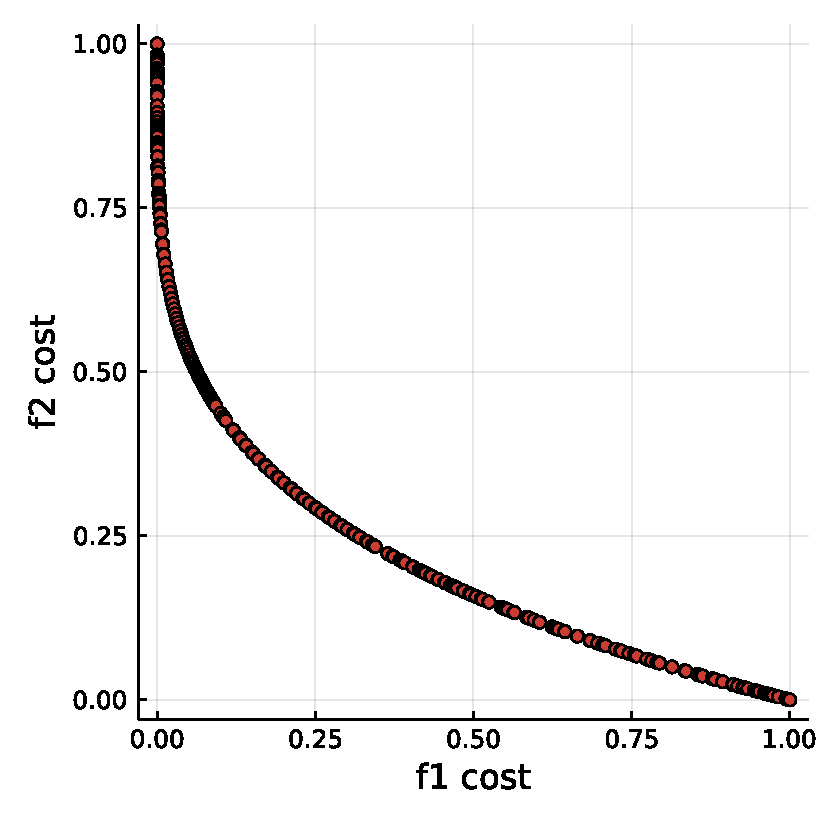
\includegraphics[width=12cm]{fig/cvx2.pdf}
      \cprotect\caption{Pareto front for F5.1}
      % \label{fig:ZDT1}
      \end{figure}

   \subsubsection{F5.2~\cite{audet2008multiobjective}}
      \textbf{Dimension of variables: }$m=2$\\
  \noindent\textbf{Problem Statement: }
   \begin{equation}
  \begin{aligned}
  f_1(x_1) &= 4x_1 \\
  g\left(x_{2}\right)&= \begin{cases}4-3 \exp \left(-(\frac{x_{2}-0.2}{0.02})^{2}\right) & \text { if } 0 \leq x_{2} \leq 0.4 \\ 4-2 \exp \left(-(\frac{x_{2}-0.7}{0.2})^{2}\right) & \text { if } 0.4 \leq x_{2} \leq 1\end{cases}\\
  h\left(f_{1}, g\right)&= \begin{cases}1 -\left(\frac{f_{1}}{g}\right)^{4} & \text { if } f_{1} \leq g \\ 0 & \text { otherwise }\end{cases}\\
  f_2(x_{1}, x_{2})&=g\cdot h
  \end{aligned}
  \end{equation}
  \noindent\textbf{Constraints: } $x_{1}, x_{2} \in[0,1]$\\
  \noindent\textbf{Features: } Concave\\
  \noindent\textbf{Hypervolume: } 0.68\\
  \noindent\textbf{Pareto front}
      \begin{figure}[H]
      \centering
      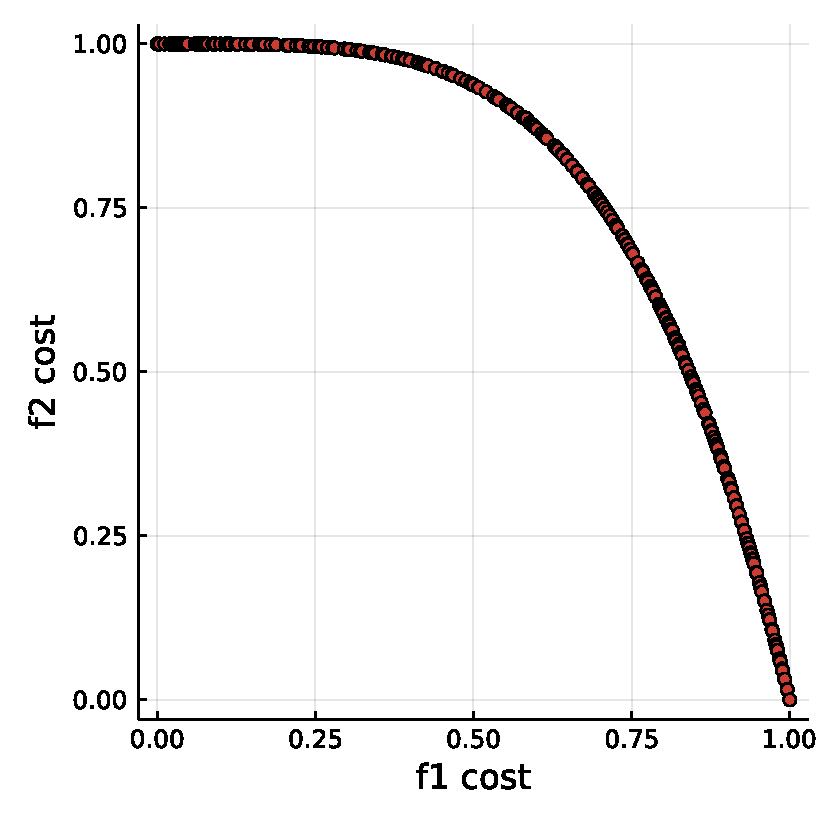
\includegraphics[width=12cm]{fig/ncvx2.pdf}
      \cprotect\caption{Pareto front for F5.2}
      % \label{fig:ZDT1}
      \end{figure}
   \subsubsection{F5.3~\cite{audet2008multiobjective}}
    \textbf{Dimension of variables: }$m=2$\\
  \noindent\textbf{Problem Statement: }
   \begin{equation}
  \begin{aligned}
  f_1(x_1) &= x_1 \\
  g(x_2) &= 1 + 10x_2\\
  h\left(f_{1}, g\right)&=1-\left(\frac{f_{1}}{a}\right)^{2}-\frac{f_{1}}{g} \sin \left(8 \pi f_{1}\right)\\
  f_2(x_{1}, x_{2})&=g\cdot h
  \end{aligned}
  \end{equation}
  \noindent\textbf{Constraints: } $x_{1}, x_{2} \in[0,1]$\\
  \noindent\textbf{Features: } Discontinuous\\
  \noindent\textbf{Hypervolume: } 0.85\\
  \noindent\textbf{Pareto front}
      \begin{figure}[H]
      \centering
      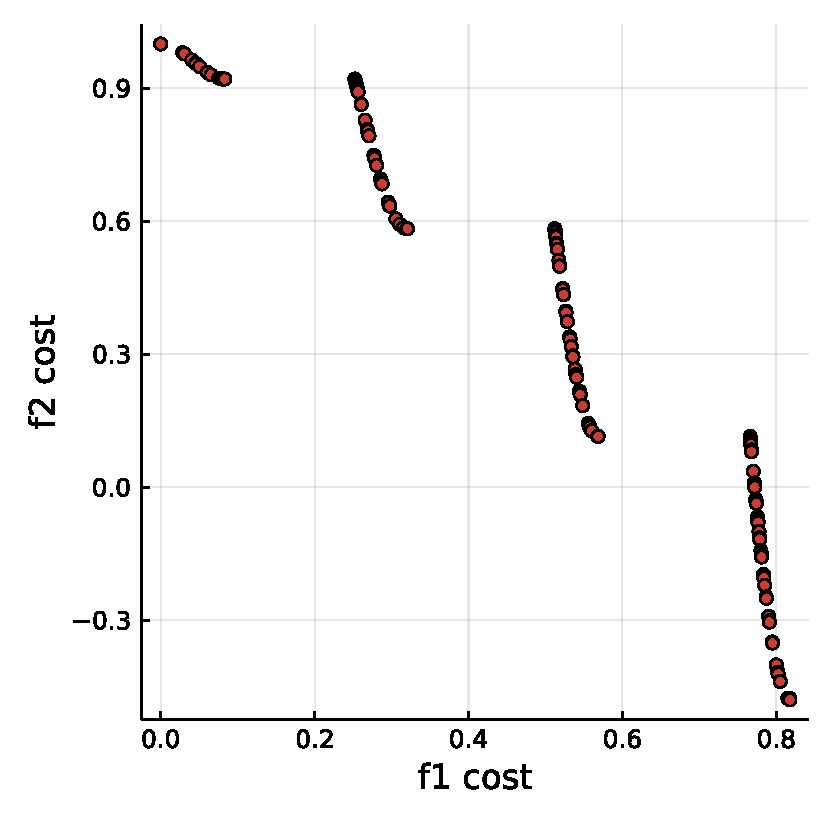
\includegraphics[width=12cm]{fig/dt2.pdf}
      \cprotect\caption{Pareto front for F5.3}
      % \label{fig:ZDT1}
      \end{figure}


   \subsubsection{F5.4~\cite{audet2008multiobjective}}
     \textbf{Dimension of variables: }$m=2$\\
  \noindent\textbf{Problem Statement: }
   \begin{equation}
  \begin{aligned}
  f_1(x_1) &= x_1 \\
  g\left(x_{2}\right)&=1+x_{2}^{0.25}\\
  h\left(f_{1}, g\right)&=1-\left(\frac{f_{1}}{g}\right)^{2}\\
  f_2(x_{1}, x_{2})&=g\cdot h
  \end{aligned}
  \end{equation}
  \noindent\textbf{Constraints: } $x_{1}, x_{2} \in[0,1]$\\
  \noindent\textbf{Features: } Concave, Bias: non-uniform search space. \\
  \noindent\textbf{Hypervolume: } 0.89\\
  \noindent\textbf{Pareto front}
      \begin{figure}[H]
      \centering
      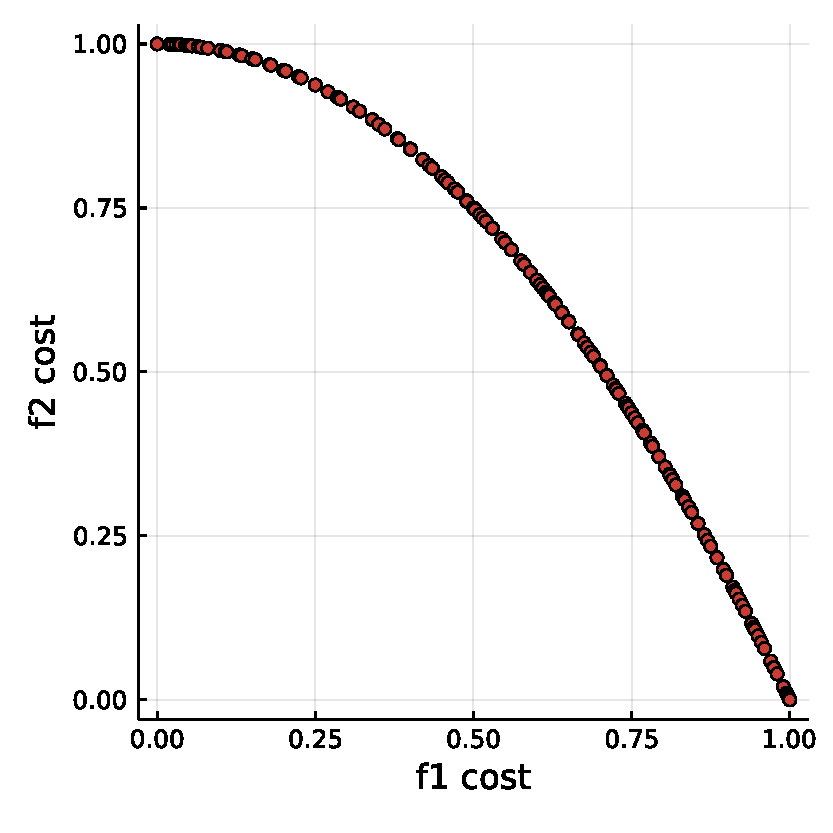
\includegraphics[width=12cm]{fig/bias.pdf}
      \cprotect\caption{Pareto front for F5.4}
      % \label{fig:ZDT1}
      \end{figure}

   \subsubsection{F5.5~\cite{audet2008multiobjective}}
      \textbf{Dimension of variables: }$m=2$\\
  \noindent\textbf{Problem Statement: }
   \begin{equation}
   \begin{aligned}
  f_{1}\left(x_{1}\right) &=1-\exp \left(-4 x_{1}\right) \sin ^{4}\left(5 \pi x_{1}\right) \\
  h\left(f_{1}, g\right) &= \begin{cases}1-\left(\frac{f_{1}}{g}\right)^{4} & \text { if } f_{1} \leq g, \\
  0 & \text { otherwise }\end{cases} \\
  g\left(x_{2}\right)&= \begin{cases}4-3 \exp \left(-\frac{x_{2}-0.2}{0.02}\right)^{2} & \text { if } 0 \leq x_{2} \leq 0.4 \\
  4-2 \exp \left(-\frac{x_{2}-0.7}{0.2}\right)^{2} & \text { if } 0.4 \leq x_{2} \leq 1\end{cases}\\
  f_2(x_{1}, x_{2})&=g\cdot h
  \end{aligned}
  \end{equation}
  \noindent\textbf{Constraints: } $x_{1}, x_{2} \in[0,1]$\\
  \noindent\textbf{Features: } Concave, Non-uniform: density of the solutions is lowest near the Pareto front.\\
  \noindent\textbf{Hypervolume: } 1.861\\
  \noindent\textbf{Pareto front}
      \begin{figure}[H]
      \centering
      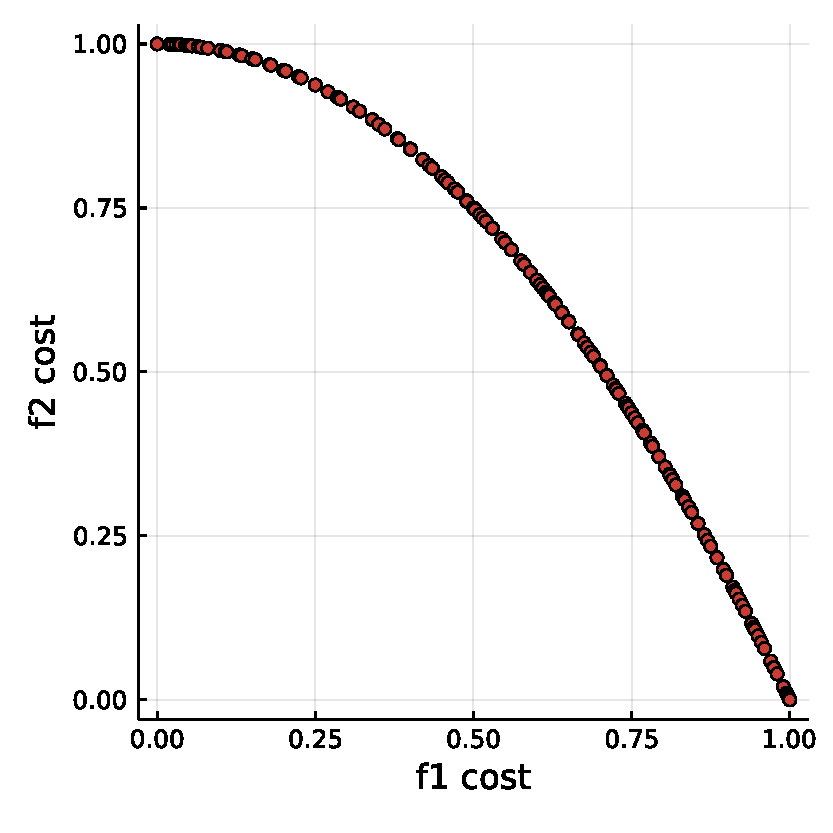
\includegraphics[width=12cm]{fig/bias.pdf}
      \cprotect\caption{Pareto front for F5.4}
      % \label{fig:ZDT1}
      \end{figure}

   \subsubsection{F1~\cite{brockhoff2016using}}
       \textbf{Dimension of variables: }$m=5$\\
  \noindent\textbf{Problem Statement: }
   \begin{equation}
   \begin{aligned}
  f_{1}(\mathbf{x})&=\left(\sum_{i}^m x_{i}^{2}\right)^{2}-20\\
  f_{2}(\mathbf{x})&=\left(\sum_{i}^m x_{i}^{2}\right)^{2}-10
  \end{aligned}
  \end{equation}
  \noindent\textbf{Constraints: } $x_{1}, \cdots,x_{m} \in[-5,5]$\\
  \noindent\textbf{Features: } Convex\\
  \noindent\textbf{Hypervolume: } 1.20\\
  \noindent\textbf{Pareto front}
      \begin{figure}[H]
      \centering
      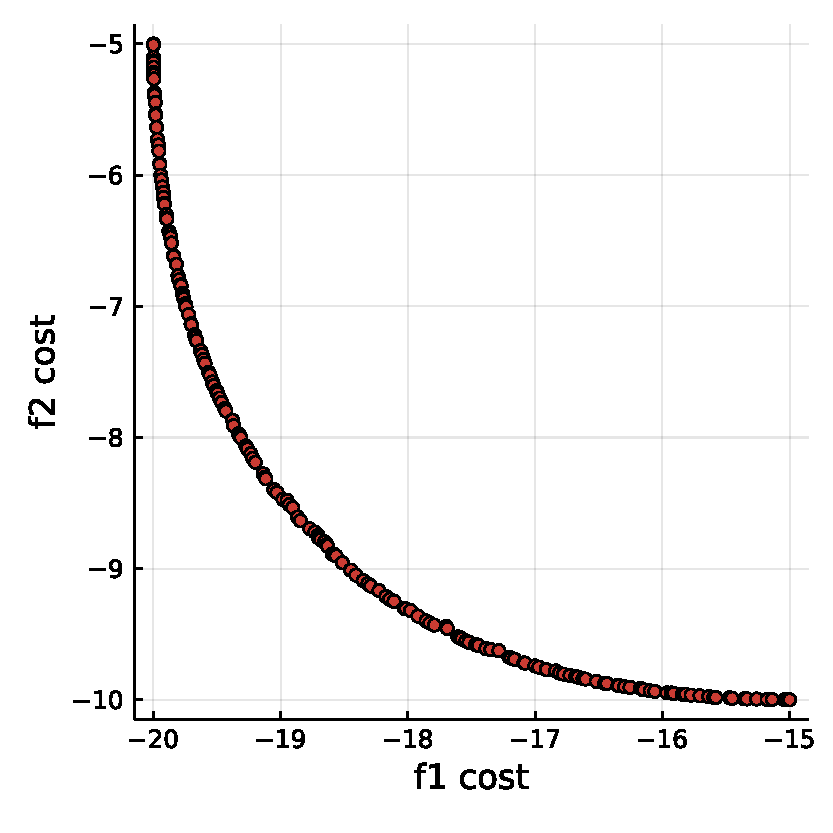
\includegraphics[width=12cm]{fig/F1.pdf}
      \cprotect\caption{Pareto front for F1}
      % \label{fig:ZDT1}
      \end{figure}

   \subsubsection{DTLZ1~\cite{huband2006review}}
     \textbf{Dimension of variables: }$m=2$\\
  \noindent\textbf{Problem Statement: }
   \begin{equation}
   \begin{aligned}
  g(x_1) &=100\left[1+\left(x_{1}-0.5\right)^{2}-\cos \left(20 \pi\left(x_{1}-0.5\right)\right)\right]\\
  f_{1}(x_1)&=(1+g)\cdot 0.5\cdot x_{1}\\
  f_2(x_1,x_2)&=0.5 \cdot(1 + g) \cdot x_1 \cdot (1 - x_2)
  \end{aligned}
  \end{equation}
  \noindent\textbf{Constraints: } $x_{1}, x_{2} \in[0,1]$\\
  \noindent\textbf{Features: } Multimodality, linear\\
  \noindent\textbf{Hypervolume: } 1.17\\
  \noindent\textbf{Pareto front}
      \begin{figure}[H]
      \centering
      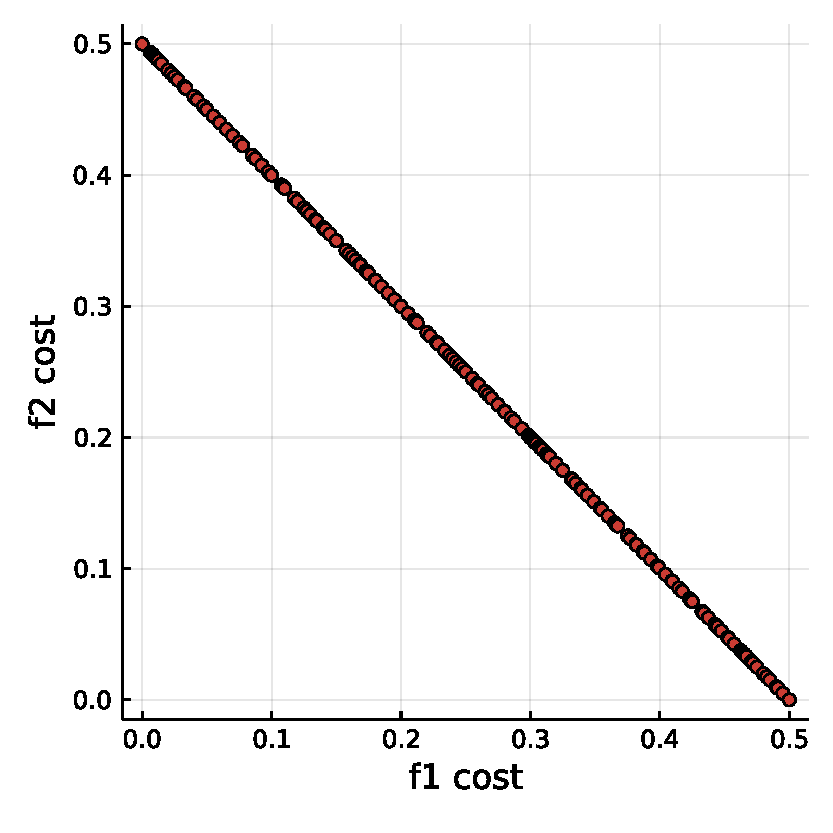
\includegraphics[width=12cm]{fig/DTLZ1n2.pdf}
      \cprotect\caption{Pareto front for DTLZ1}
      % \label{fig:ZDT1}
      \end{figure}


  \subsubsection{MOP2~\cite{huband2006review}}
   \textbf{Dimension of variables: }$m=3$\\
  \noindent\textbf{Problem Statement: }

  \begin{equation}
  \begin{aligned}
  f_{1}\left(x_{1}, \ldots, x_{m}\right) &=1-\exp \left(-\sum_{i=1}^{m}\left(x_{i}-1 / \sqrt{m}\right)^{2}\right) \\
  f_{2}\left(x_{1}, \ldots, x_{m}\right) &=1-\exp \left(-\sum_{i=1}^{m}\left(x_{i}+1 / \sqrt{m}\right)^{2}\right)
  \end{aligned}
  \end{equation}

  \noindent\textbf{Constraints: } $x_{1},\cdots , x_{m} \in[-4,4]$\\
  \noindent\textbf{Features: } Concave\\
  \noindent\textbf{Hypervolume: } 0.86\\
  \noindent\textbf{Pareto front}
      \begin{figure}[H]
      \centering
      \includegraphics[width=12cm]{fig/mop2.pdf}
      \cprotect\caption{Pareto front for MOP2}
      % \label{fig:ZDT1}
      \end{figure}


   \subsubsection{MOP3~\cite{huband2006review}}
   \textbf{Dimension of variables: }$m=2$\\
  \noindent\textbf{Problem Statement: }

  \begin{equation}
  \begin{aligned}
  f_{1}\left(x_{1}, x_{2}\right) &=1+\left(A_{1}-B_{1}\right)^{2}+\left(A_{2}-B_{2}\right)^{2} \\
  f_{2}\left(x_{1}, x_{2}\right) &=\left(x_{1}+3\right)^{2}+\left(x_{2}+1\right)^{2} \\
  A_{1} &=0.5 \sin (1)-2 \cos (1)+\sin (2)-1.5 \cos (2) \\
  A_{2} &=1.5 \sin (1)-\cos (1)+2 \sin (2)-0.5 \cos (2) \\
  B_{1} &=0.5 \sin (x_{1})-2 \cos (x_{1})+\sin (x_{2})-1.5 \cos (x_{2}) \\
  B_{2} &=1.5 \sin (x_{1})-1 \cos (x_{1})+2 \sin (x_{2})-0.5 \cos (x_{2})
  \end{aligned}
  \end{equation}

  \noindent\textbf{Constraints: } $x_{1}, x_{2} \in[-\pi,\pi]$\\
  \noindent\textbf{Features: } Discontinuous, Convex\\
  \noindent\textbf{Hypervolume: } 1.85\\
  \noindent\textbf{Pareto front}
      \begin{figure}[H]
      \centering
      \includegraphics[width=11cm]{fig/mop3.pdf}
      \cprotect\caption{Pareto front for MOP3}
      % \label{fig:ZDT1}
      \end{figure}

  \subsubsection{MOP4~\cite{huband2006review}}\label{sec:mop4}
  % A degenerate points
   \textbf{Dimension of variables: }$m=3$\\
  \noindent\textbf{Problem Statement: }

  \begin{equation}
  \begin{aligned}
  f_{1}\left(x_{1}, \cdots, x_{m}\right) &=\sum_{i=1}^{2}-10 \exp ^{-0.2 \sqrt{x_{i}^{2}+x_{i+1}^{2}}} \\
  f_{2}\left(x_{1}, \cdots, x_{m}\right) &=\sum_{i=1}^{3}\left|x_{i}\right|^{0.8}+5 \sin \left(x_{i}^{3}\right)
  \end{aligned}
  \end{equation}

  \noindent\textbf{Constraints: } $x_{1},\cdots , x_{m} \in[-5,5]$\\
  \noindent\textbf{Features: } Degenerate points (single point on the Pareto front), Mixed front\\
  \noindent\textbf{Hypervolume: } 0.642\\
  \noindent\textbf{Pareto front}
      \begin{figure}[H]
      \centering
      \includegraphics[width=12cm]{fig/mop4.pdf}
      \cprotect\caption{Pareto front for MOP4}
      % \label{fig:ZDT1}
      \end{figure}

   \subsubsection{MOP6~\cite{huband2006review}}
   \textbf{Dimension of variables: }$m=2$\\
  \noindent\textbf{Problem Statement: }

  \begin{equation}
  \begin{aligned}
  f_{1}\left(x_{1}\right) &=x_{1} \\
  f_{2}\left(x_{1}, x_{2}\right) &=\left(1+10 x_{2}\right)\left(1-\left(\frac{x_{1}}{1+10 x_{2}}\right)^{2}-\frac{x_{1}}{1+10 x_{2}} \sin \left(8 \pi x_{1}\right)\right)
  \end{aligned}
  \end{equation}

  \noindent\textbf{Constraints: } $x_{1}, x_{2} \in[0,1]$\\
  \noindent\textbf{Features: } Discontinuous, Multimodality, Mixed front\\
  \noindent\textbf{Hypervolume: } 0.80\\
  \noindent\textbf{Pareto front}
      \begin{figure}[H]
      \centering
      \includegraphics[width=12cm]{fig/mop6.pdf}
      \cprotect\caption{Pareto front for MOP4}
      % \label{fig:ZDT1}
      \end{figure}

   \subsubsection{FES1~\cite{huband2006review}}
   \textbf{Dimension of variables: }$m=10$\\
  \noindent\textbf{Problem Statement: }

  \begin{equation}
  \begin{aligned}
  f_{1}\left(x_{1}, \ldots, x_{m}\right)&=\sum_{i=1}^{m}\left|x_{i}-\exp \left((i / m)^{2}\right) / 3\right|^{0.5} \\
  f_{2}\left(x_{1}, \ldots, x_{m}\right)&=\sum_{i=1}^{m}\left(x_{i}-0.5 \cos (10 \pi i / m)-0.5\right)^{2}
  \end{aligned}
  \end{equation}

  \noindent\textbf{Constraints: } $x_{1},\cdots , x_{m} \in[0,1]$\\
  \noindent\textbf{Features: } Mixed front\\
  \noindent\textbf{Hypervolume: } 0.80\\
  \noindent\textbf{Pareto front}
      \begin{figure}[H]
      \centering
      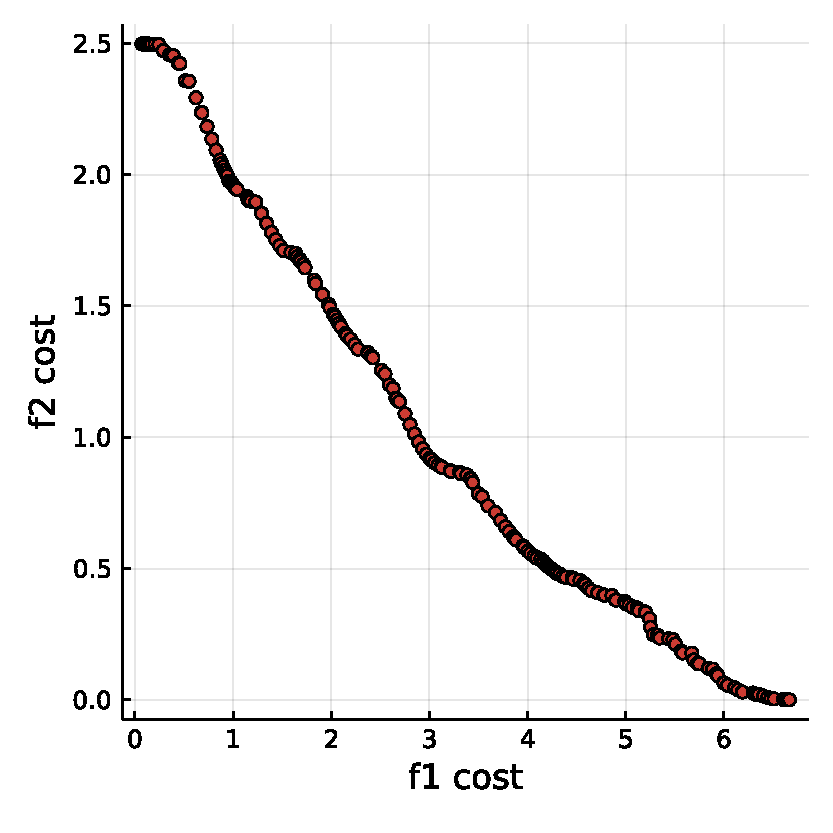
\includegraphics[width=12cm]{fig/FES1.pdf}
      \cprotect\caption{Pareto front for FES1}
      % \label{fig:ZDT1}
      \end{figure}

   \subsubsection{QV1~\cite{huband2006review}}
   \textbf{Dimension of variables: }$m=10$\\
  \noindent\textbf{Problem Statement: }

  \begin{equation}
  \begin{aligned}
  f_{1}\left(x_{1}, \ldots, x_{m}\right) &=\left[\sum_{i=1}^{m}\left(x_{i}^{2}-10 \cos \left(2 \pi x_{i}\right)+10\right) / m\right]^{0.25} \\
  f_{2}\left(x_{1}, \ldots, x_{m}\right) &=\left[\sum_{i=1}^{m}\left(\left(x_{i}-1.5\right)^{2}-10 \cos \left(2 \pi\left(x_{i}-1.5\right)\right)+10\right) / m\right]^{0.25}
  \end{aligned}
  \end{equation}

  \noindent\textbf{Constraints: } $x_{1},\cdots , x_{m} \in[0,1]$\\
  \noindent\textbf{Features: } Multimodality, Concave\\
  \noindent\textbf{Hypervolume: } 0.87\\
  \noindent\textbf{Pareto front}
      \begin{figure}[H]
      \centering
      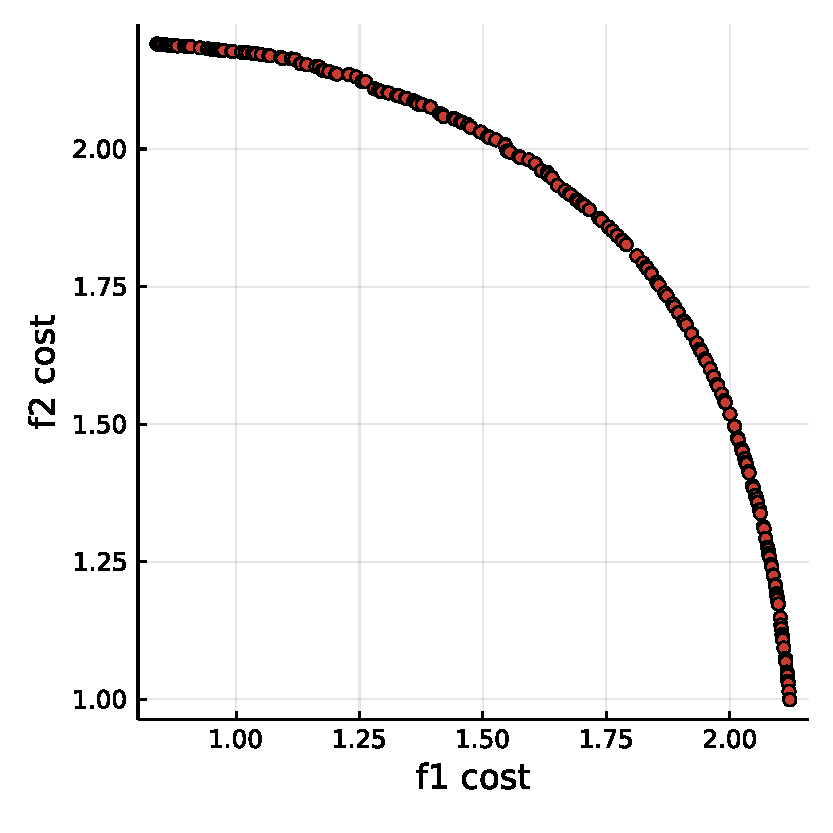
\includegraphics[width=12cm]{fig/QV1.pdf}
      \cprotect\caption{Pareto front for QV1}
      % \label{fig:ZDT1}
      \end{figure}


   \subsubsection{OKA1~\cite{davidor1994parallel}}
   \textbf{Dimension of variables: }$m=2$\\
  \noindent\textbf{Problem Statement: }

  \begin{equation}
  \begin{aligned}
  y_1 &= x_1\cdot \cos(\pi/12)   - x_2\cdot \sin(\pi/12)   \\
      y_2 &=x_1\cdot \sin(\pi/12)   +x_2\cdot \cos(\pi/12) \\
      f_1(x_1, x_2) &= y_1 \\
      f_2(x_1,x_2) &= \sqrt{2\pi} - \sqrt{|y_1|} + 2  |y_2 - 3 \cos(y_1) - 3|^{1/3}
  \end{aligned}
  \end{equation}

  \noindent\textbf{Constraints: } $x_1\in [6\sin(\pi/12), 6\sin(\pi/12)+2\pi \cos(\pi/12)]$, $x_2\in [-2\pi \sin(\pi/12), 6\cos(\pi/12)]$\\
  \noindent\textbf{Features: } Non-uniform\\
  \noindent\textbf{Hypervolume: } 0.80\\
  \noindent\textbf{Pareto front}
      \begin{figure}[H]
      \centering
      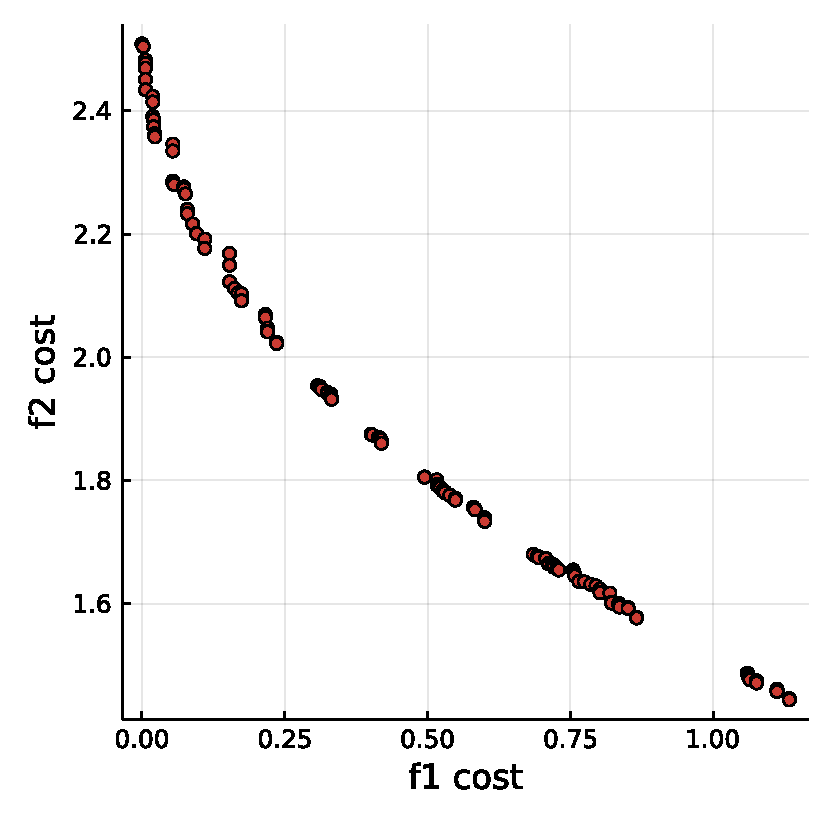
\includegraphics[width=12cm]{fig/OKA1.pdf}
      \cprotect\caption{Pareto front for OKA1}
      % \label{fig:ZDT1}
      \end{figure}

   \subsubsection{FAR1~\cite{huband2006review}}
   \textbf{Dimension of variables: }$m=2$\\
  \noindent\textbf{Problem Statement: }

  \begin{equation}
  \begin{aligned}
  f_{1}\left(x_{1}, x_{2}\right)=&-2 \exp \left(15\left(-\left(x_{1}-0.1\right)^{2}-x_{2}^{2}\right)\right)-\exp \left(20\left(-\left(x_{1}-0.6\right)^{2}-\left(x_{2}-0.6\right)^{2}\right)\right) \\
  &+\exp \left(20\left(-\left(x_{1}+0.6\right)^{2}-\left(x_{2}-0.6\right)^{2}\right)\right)+\exp \left(20\left(-\left(x_{1}-0.6\right)^{2}-\left(x_{2}+0.6\right)^{2}\right)\right) \\
  &+\exp \left(20\left(-\left(x_{1}+0.6\right)^{2}-\left(x_{2}+0.6\right)^{2}\right)\right) \\
  f_{2}\left(x_{1}, x_{2}\right)=& 2 \exp \left(20\left(-x_{1}^{2}-x_{2}^{2}\right)\right) +\exp \left(20\left(-\left(x_{1}-0.4\right)^{2}-\left(x_{2}-0.6\right)^{2}\right)\right) \\
  &-\exp \left(20\left(-\left(x_{1}+0.5\right)^{2}-\left(x_{2}-0.7\right)^{2}\right)\right)-\exp \left(20\left(-\left(x_{1}-0.5\right)^{2}-\left(x_{2}+0.7\right)^{2}\right)\right) \\
  &+\exp \left(20\left(-\left(x_{1}+0.4\right)^{2}-\left(x_{2}+0.8\right)^{2}\right)\right)
  \end{aligned}
  \end{equation}

  \noindent\textbf{Constraints: } $x_1, x_2\in [0,1]$\\
  \noindent\textbf{Features: } Mixed front\\
  \noindent\textbf{Hypervolume: } 0.27\\
  \noindent\textbf{Pareto front}
      \begin{figure}[H]
      \centering
      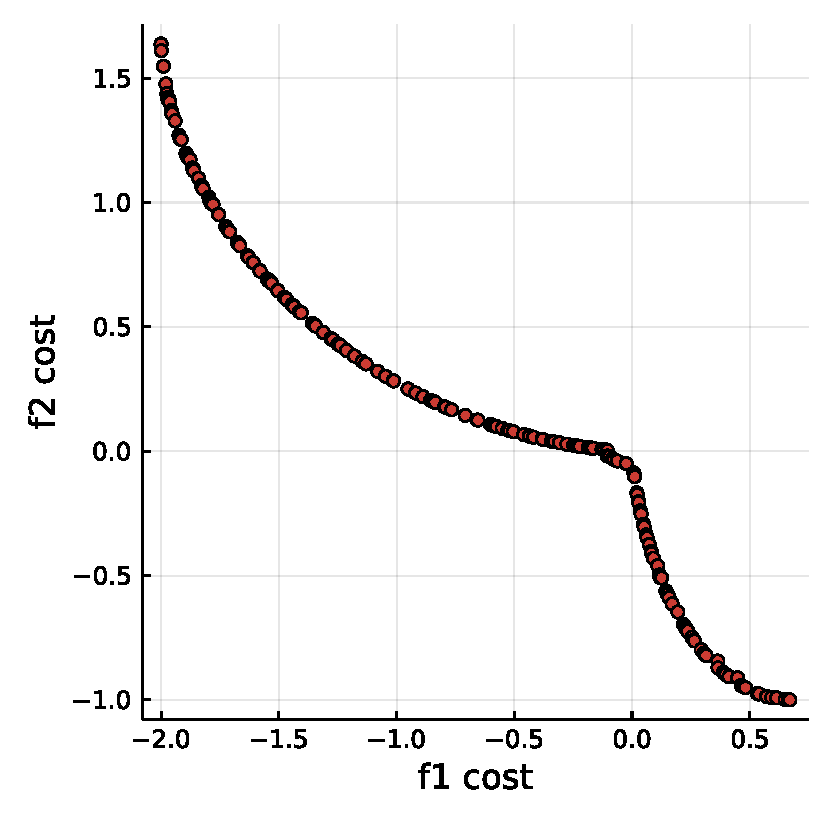
\includegraphics[width=10cm]{fig/FAR1.pdf}
      \cprotect\caption{Pareto front for FAR1}
      % \label{fig:ZDT1}
      \end{figure}


\newpage
\subsection{Parameters for Building Case}\label{sec:parameter}
\begin{equation}
A=-\left(a U+V c_{\text {air }} \rho_{\text {air }} n_{\text {ac }}\right)
\end{equation}
% Table generated by Excel2LaTeX from sheet 'Sheet1'
\begin{table}[t]
  \centering
  \caption{Parameters for building case}
    \begin{tabular}{clcc|clcc}
    \toprule
\textbf{Symbol} & \textbf{Global Data} & \textbf{Value} & \textbf{Unit} & \textbf{Symbol} &\textbf{Global Data} & \textbf{Value} & \textbf{Unit}\\
    \hline    
  $a$  &Wall surface area & 188.36 & $m^2$ & $U$ & Average U value & 0.65  & $W/m^2K$ \\
  $V$  &Building volume & 225   & $m^3$ & $n_{ac}$& Air changes per hour & 0.4   &  $^\circ C$ \\
   $\rho_{air}$ &Air density & 1.225 & $kg/m^3$ & $c_{air}$ & Air specific heat capacity & 1.005 & $kJ/kg\ K$  \\
    \bottomrule
    \end{tabular}%
  \label{tab:para}%
\end{table}%
\newpage
\subsection{How does BiMADS fill the gaps gradually}
 \begin{figure}[H]
  \centering
  \subfigure[Initialization]{ 
  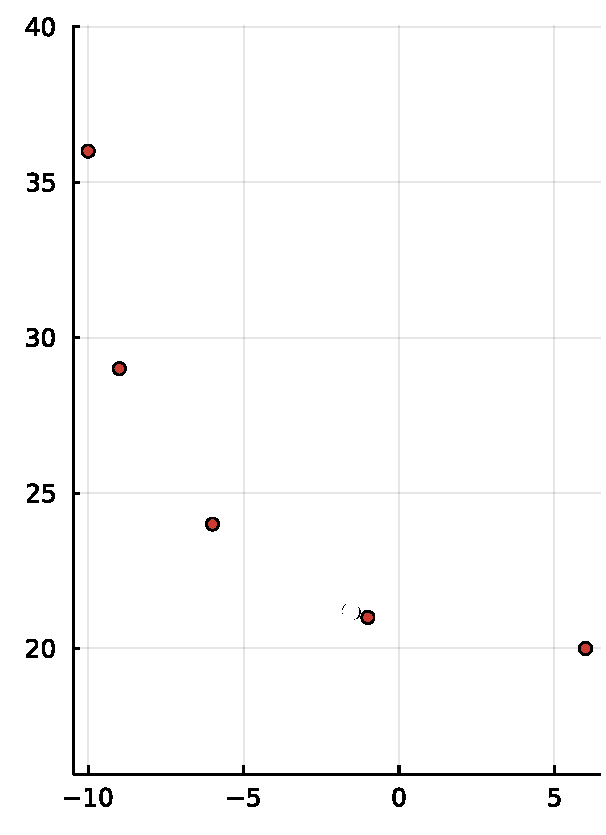
\includegraphics[width=4.4cm]{fig/DS_result_0.pdf}}
    \subfigure[Iteration 1]{ 
  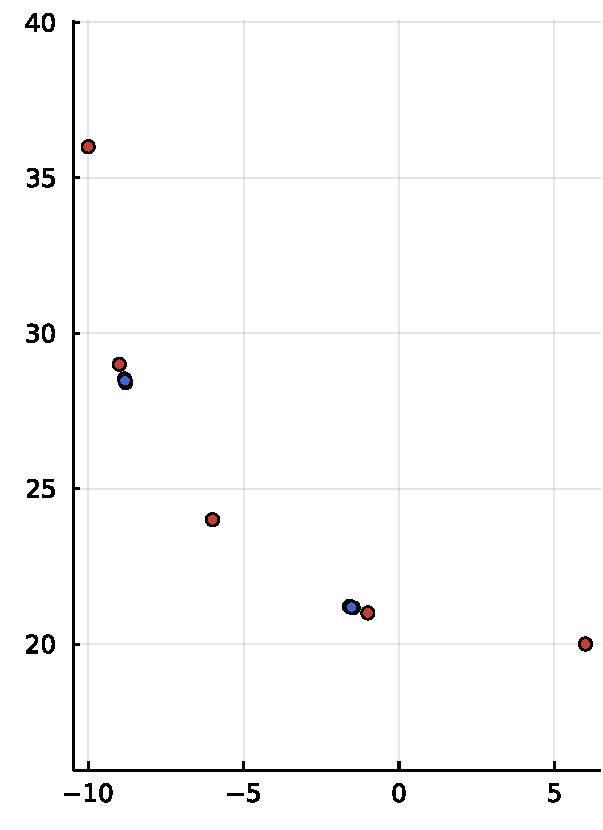
\includegraphics[width=4.4cm]{fig/DS_result_1.pdf}}
      \subfigure[Iteration 2]{ 
  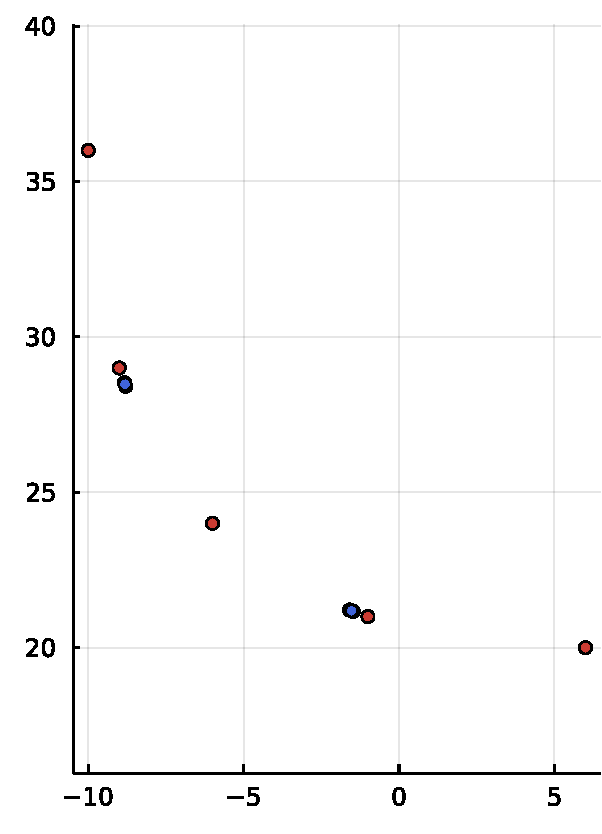
\includegraphics[width=4.4cm]{fig/DS_result_2.pdf}}\\
      \subfigure[Iteration 3]{ 
  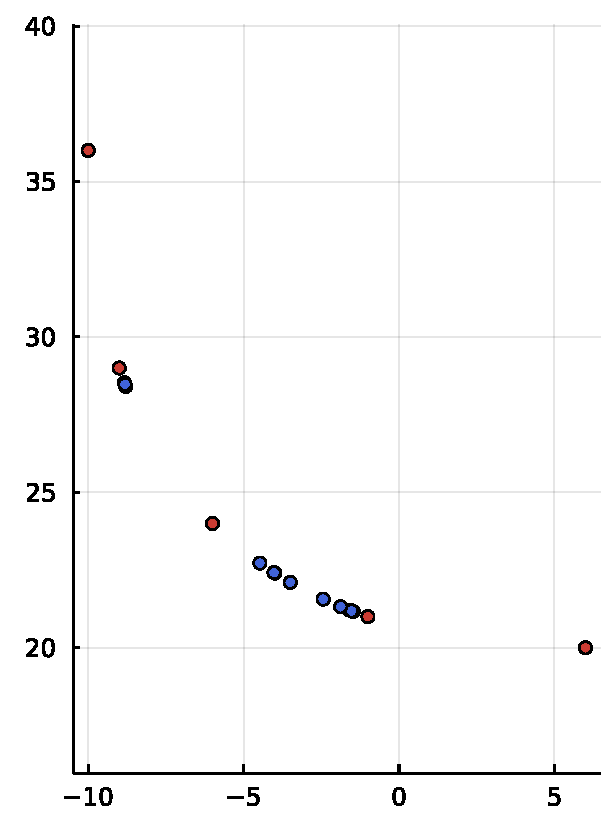
\includegraphics[width=4.4cm]{fig/DS_result_3.pdf}}
      \subfigure[Iteration 4]{ 
  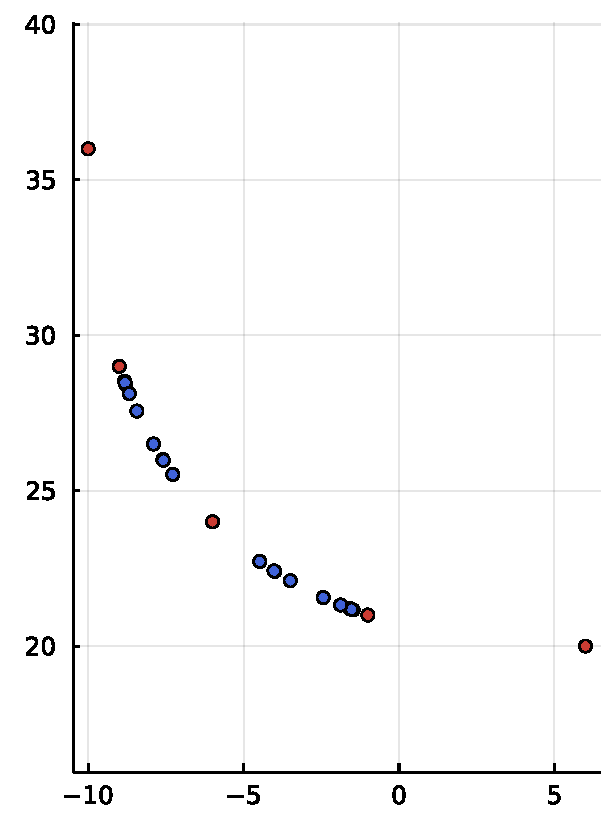
\includegraphics[width=4.4cm]{fig/DS_result_4.pdf}}
      \subfigure[Iteration 5]{ 
  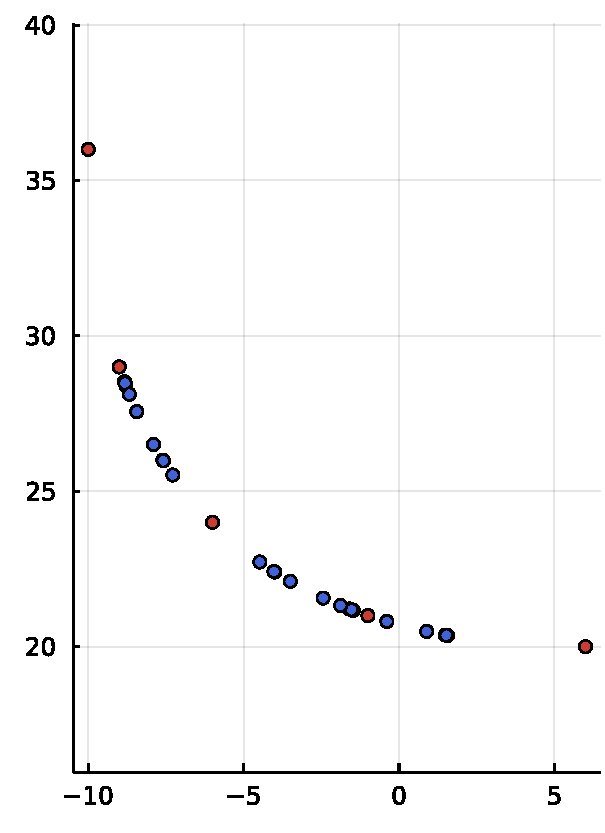
\includegraphics[width=4.4cm]{fig/DS_result_5.pdf}}\\
        \subfigure[Iteration 3]{ 
  \includegraphics[width=4.4cm]{fig/DS_result_6.pdf}}
      \subfigure[Iteration 4]{ 
  \includegraphics[width=4.4cm]{fig/DS_result_7.pdf}}
      \subfigure[Iteration 5]{ 
  \includegraphics[width=4.4cm]{fig/DS_result_8.pdf}}
  \caption{BiMADS for 500 Iterations}
  \label{fig:fillgap}
  \end{figure}




  %     \begin{listing}[ht]
  %       \begin{minted}[breaklines,escapeinside=||,mathescape=true, linenos, numbersep=3pt, gobble=2, fontsize=\small, framesep=2mm]{julia}
  % function Tref(p) #take the P,I,D values as an input
  %     P     = tf(1, [1, -A])  #transfer functions (tf) for the system
  %     C     = Kpid(p[1], p[2], p[3]) #tf for PID controller
  %     L     = feedback(P * C) |> ss #tf for feedback loop PC/(1+PC) and convert it to state-space representation
  %     #if the obtained system is improper
  %     !isproper(feedback(P * C)) && return Inf
  %     #if the obtained system is stable
  %     e,v=eigen(L.A)
  %     any(>=(0), e) && println("unstable") && return Inf

  %     #Translate the system with tf=L and input signal=ref to a manner that can be solved by an ODE solver
  %     s     = Simulator(L, ref)  
  %     ty    = eltype(p) # So that all inputs to the solver have same numerical type
  %     x0    = zeros(L.nx) .|> ty
  %     tspan = (ty(0.), ty(Tf)) #total simulation period
  %     sol   = solve(s, x0, tspan,maxiters=1e7,dtmin=0.001,reltol = 1e-1,force_dtmin=true)
  %     y     = L.C * sol(t)+ L.D .* ref #y=C*x+D*u
  %     y  # output the time response during tspan
  % end
  %     \end{minted}
  %   \cprotect\caption{System simulation in Julia for \verb|Tref|}
  %   \label{lis:tref}
  %   \end{listing}








\end{document}
